\section{\muqcd Method Validation}
\label{app:muqcd-study}
%%\paragraph{}
One important validation is wether the \muqcd is the same for different number of $b$ tags in multijet event. This can be validated in data, excluding signal regions. For data, the \ttbar contribution is estimated directly from MC and subtracted in the distributions. Then two plots are produced: one is the ratio of the number of N $b$ tagged events versus the number of N-1 $b$ tagged events in each leading Higgs candidate/subleading Higgs candiate mass bin, the second is the pull of the bins in Sideband/Control/Signal regions. The two distributions shows roughly the consistency of \muqcd in different regions, as seen in Figure~\ref{fig:app-muqcd-1b} ($1b$ over $0b$), ~\ref{fig:app-muqcd-2b} ($2b$ over $1b$), ~\ref{fig:app-muqcd-2bs} ($2b$s over $1b$), ~\ref{fig:app-muqcd-3b} ($3b$ over $2b$), ~\ref{fig:app-muqcd-4b} ($4b$ over $2b$). For $4/3/2b$s, the \muqcd value can be compared with \ref{tab:bkgfit}. In Figure ~\ref{fig:app-muqcd-1b} and ~\ref{fig:app-muqcd-2b}, \textbf{the agreement of \muqcd weighted mean value in Sideband/Control/Signal (especially) regions validates the constant \muqcd assumption in the analysis.}

%%\paragraph{}
Also, the Dijet MC can be used for validation. The same distributions, without sustracting \ttbar, are shown in Figure~\ref{fig:app-muqcd-1b-qcd} ($1b$ over $0b$), ~\ref{fig:app-muqcd-2b-qcd} ($2b$ over $1b$), ~\ref{fig:app-muqcd-2bs-qcd} ($2b$s over $1b$), ~\ref{fig:app-muqcd-3b-qcd} ($3b$ over $2b$), ~\ref{fig:app-muqcd-4b-qcd} ($4b$ over $2b$).  Poor Statistics of the dijet MC affect the pull distributions, especially for 3$b$ and 4$b$ ratios, yet the consistency of \muqcd in different regions can still be validated. \textbf{This also proves that the dijet MC could not be used directly for background estimation.}

\begin{figure*}[htbp!]
\begin{center}
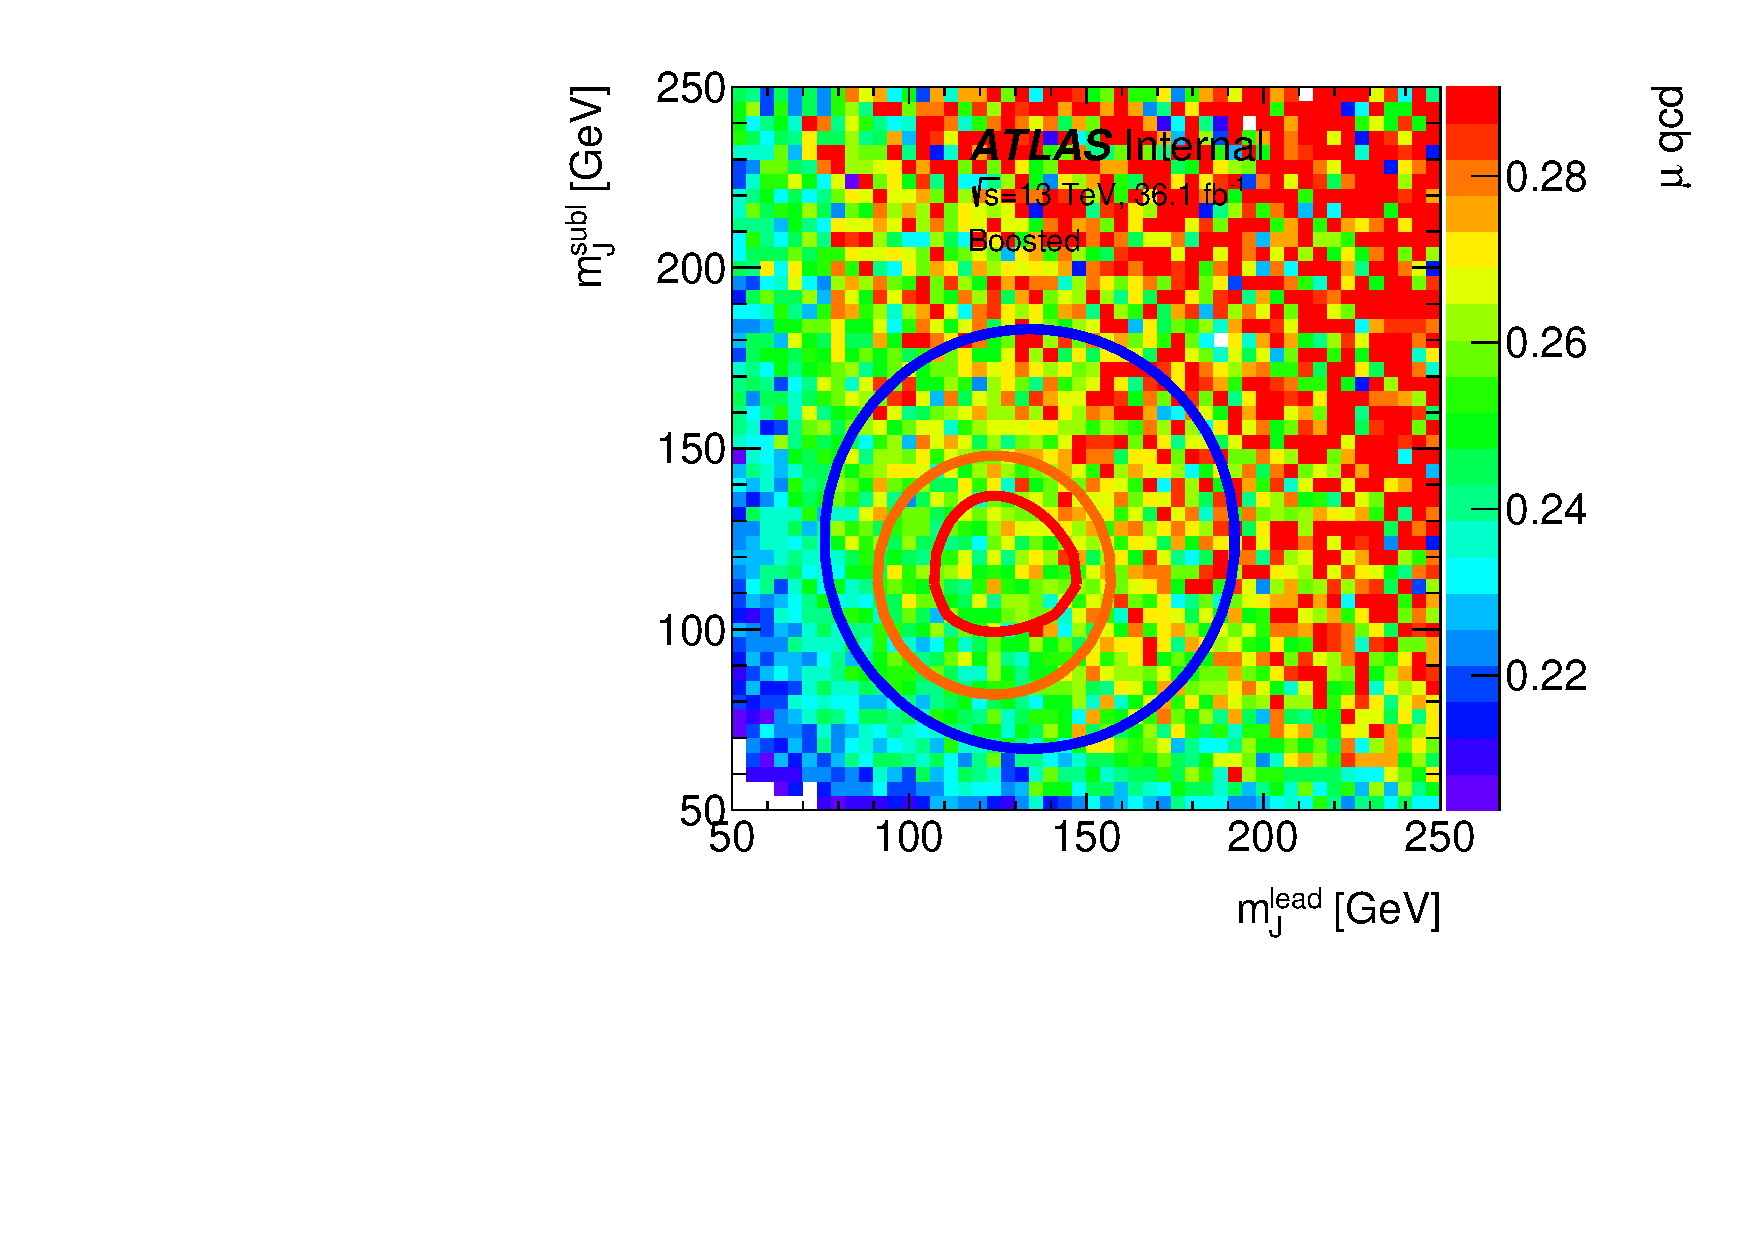
\includegraphics[width=0.45\textwidth,angle=-90]{figures/boosted/AppendixMuqcdstudy/OneTag_Incl_mH0H1.pdf}
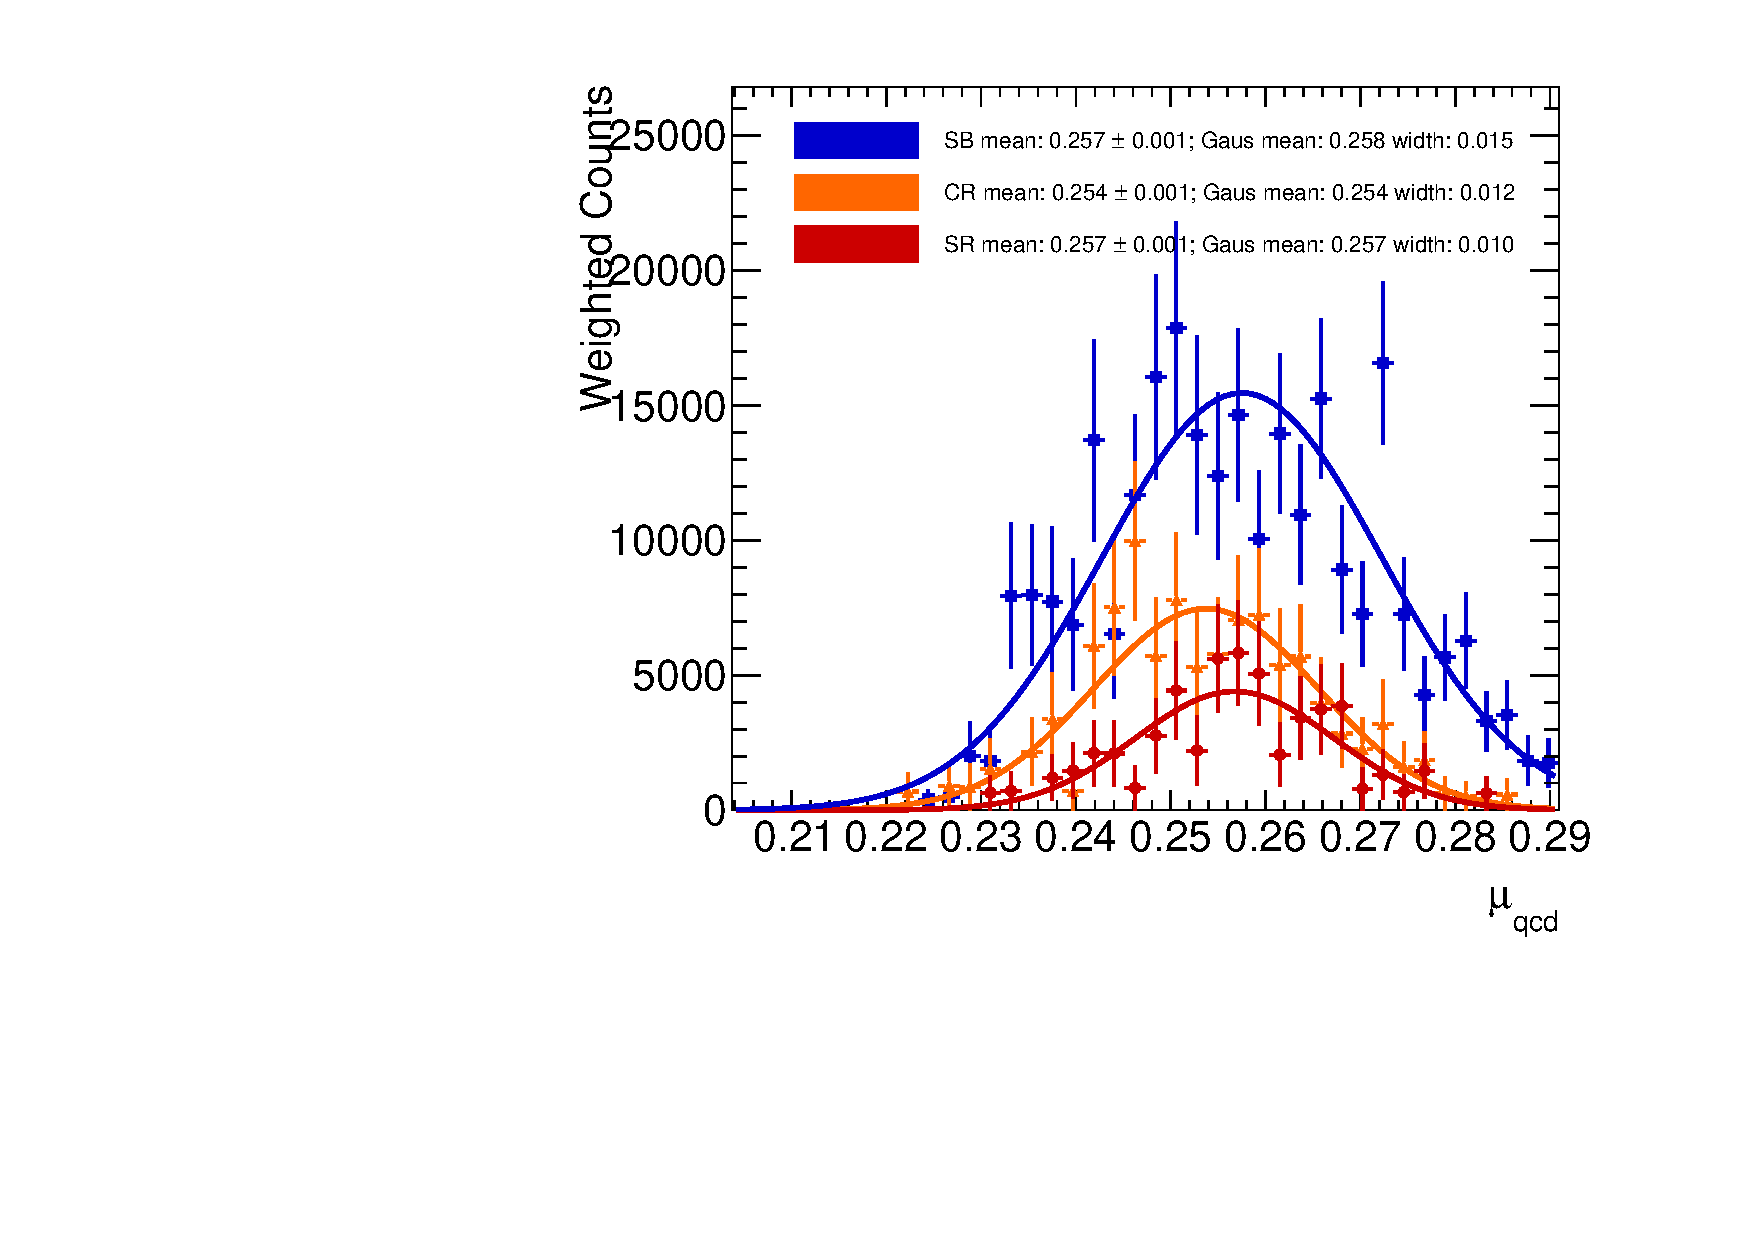
\includegraphics[width=0.45\textwidth,angle=-90]{figures/boosted/AppendixMuqcdstudy/OneTag_Incl_mH0H1_pull.pdf}
\caption{1$b$ over 0$b$ data driven \muqcd values: \muqcd as a funciton of leading Higgs candidate/subleading Higgs candiate mass(left); and \muqcd value pull in Sideband/Control/Signal regions(right), with the weighted mean value and the Guassian fit mean value shown on the plot.}
\label{fig:app-muqcd-1b}
\end{center}
\end{figure*}

\begin{figure*}[htbp!]
\begin{center}
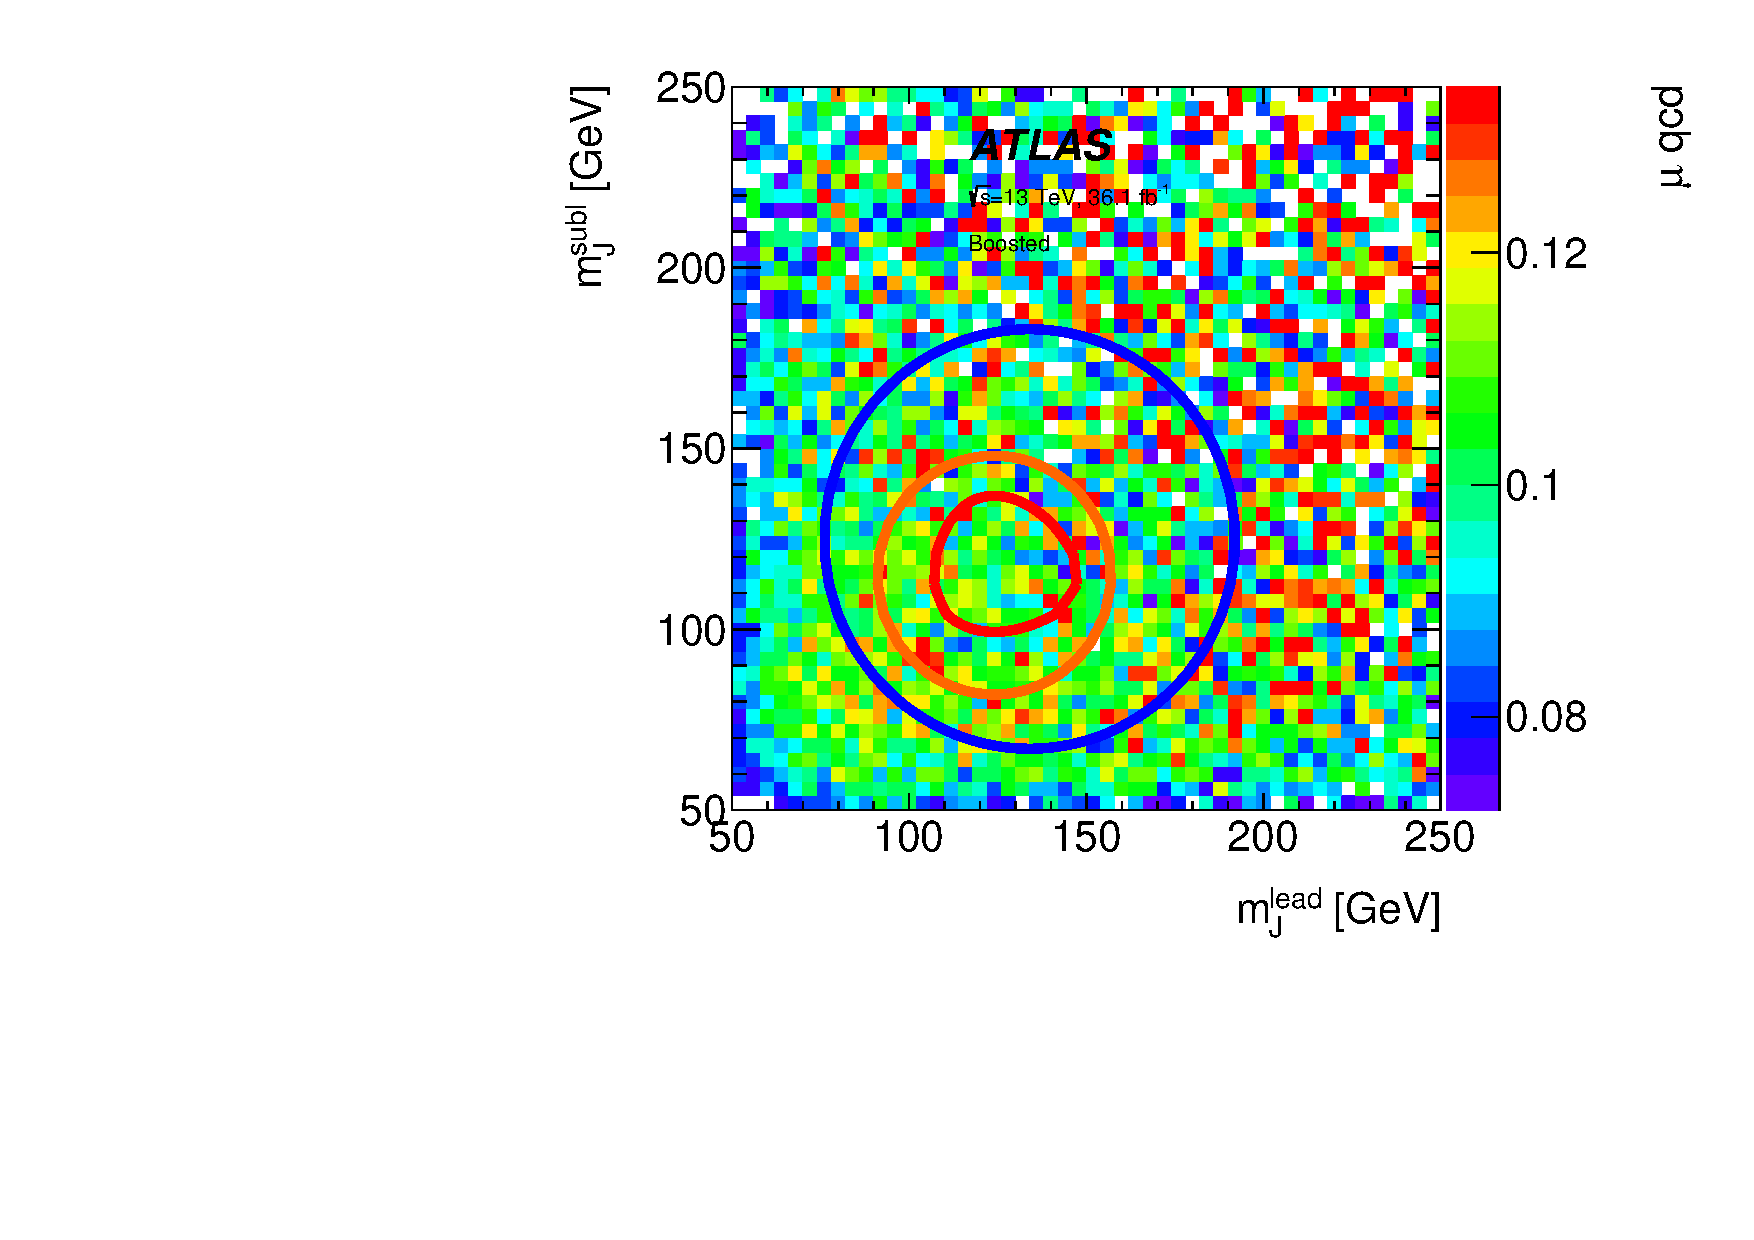
\includegraphics[width=0.45\textwidth,angle=-90]{figures/boosted/AppendixMuqcdstudy/TwoTag_Incl_mH0H1.pdf}
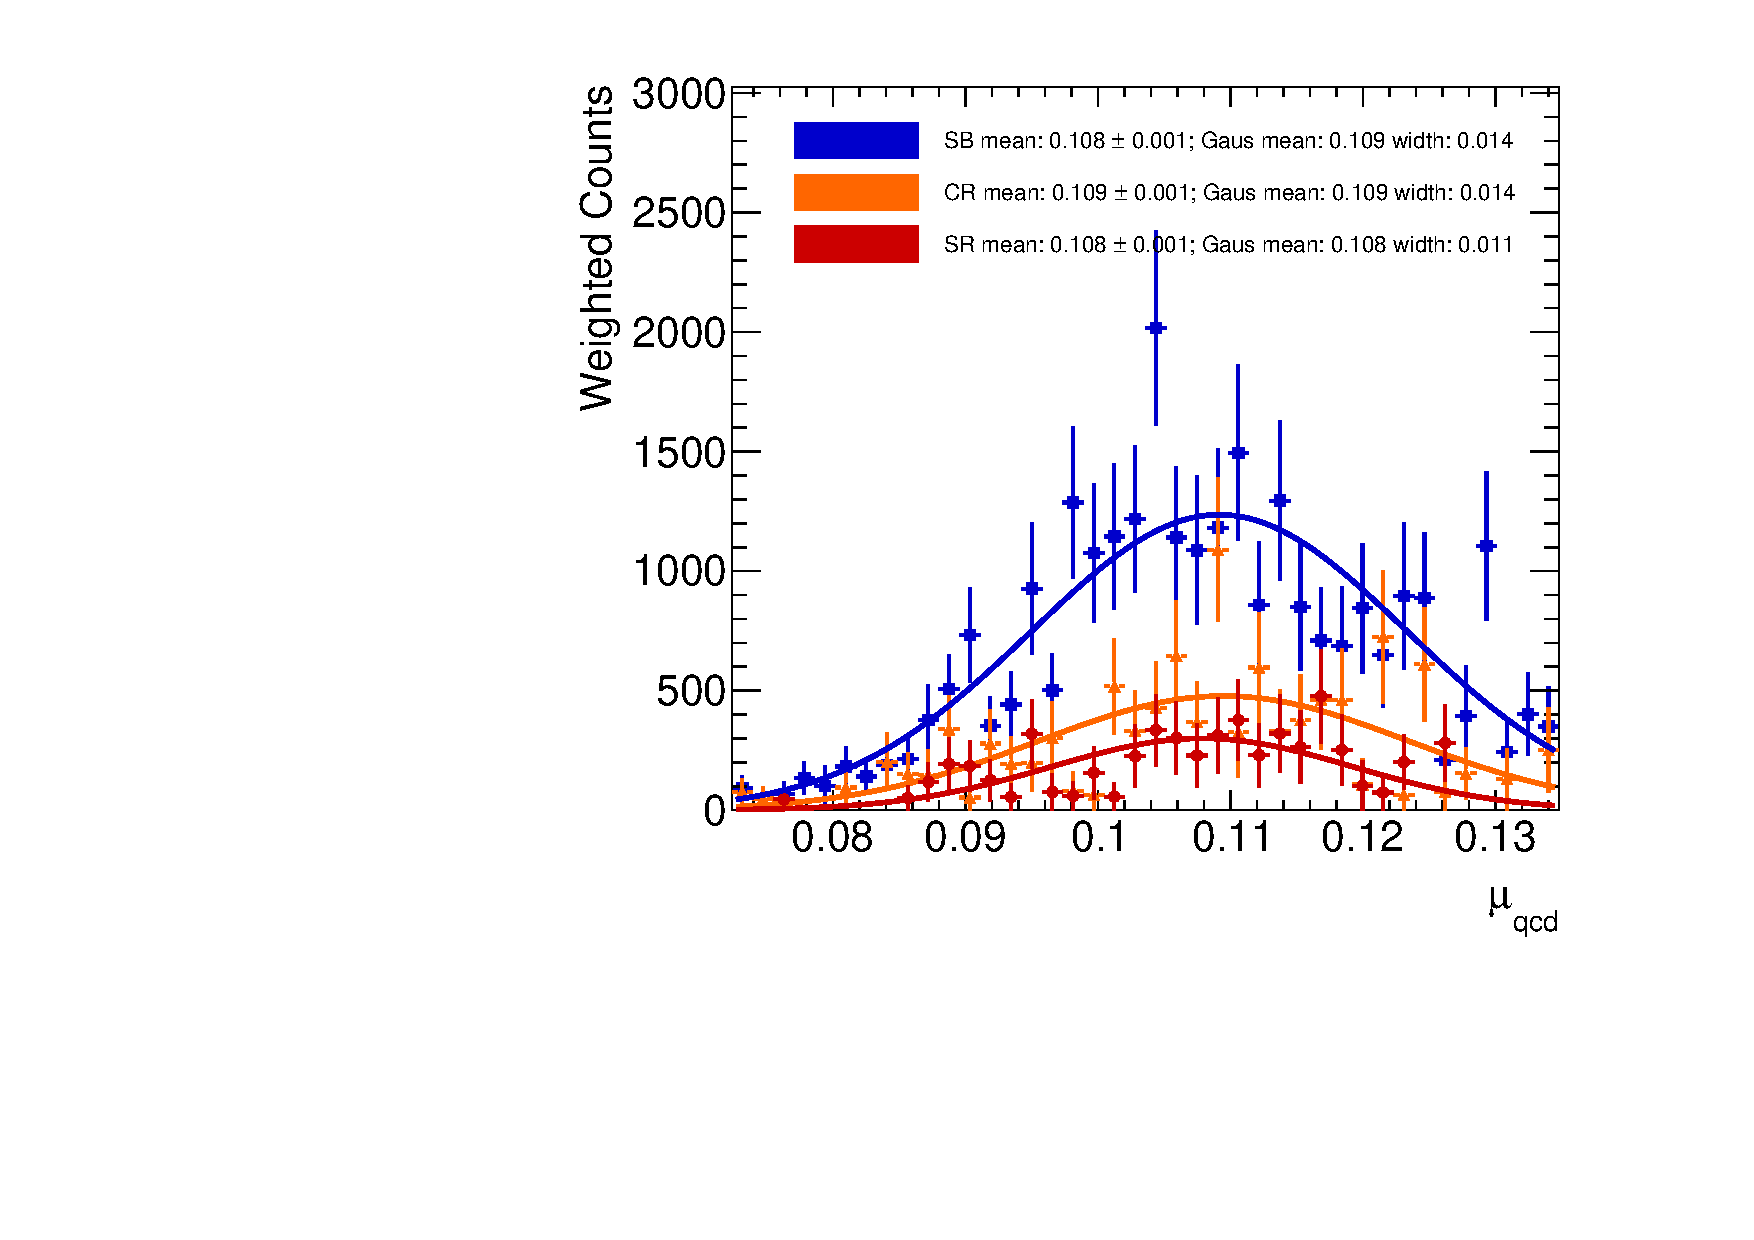
\includegraphics[width=0.45\textwidth,angle=-90]{figures/boosted/AppendixMuqcdstudy/TwoTag_Incl_mH0H1_pull.pdf}
\caption{2$b$ over 1$b$ data driven \muqcd values: \muqcd as a funciton of leading Higgs candidate/subleading Higgs candiate mass(left); and \muqcd value pull in Sideband/Control/Signal regions(right), with the weighted mean value and the Guassian fit mean value shown on the plot.}
\label{fig:app-muqcd-2b}
\end{center}
\end{figure*}

\begin{figure*}[htbp!]
\begin{center}
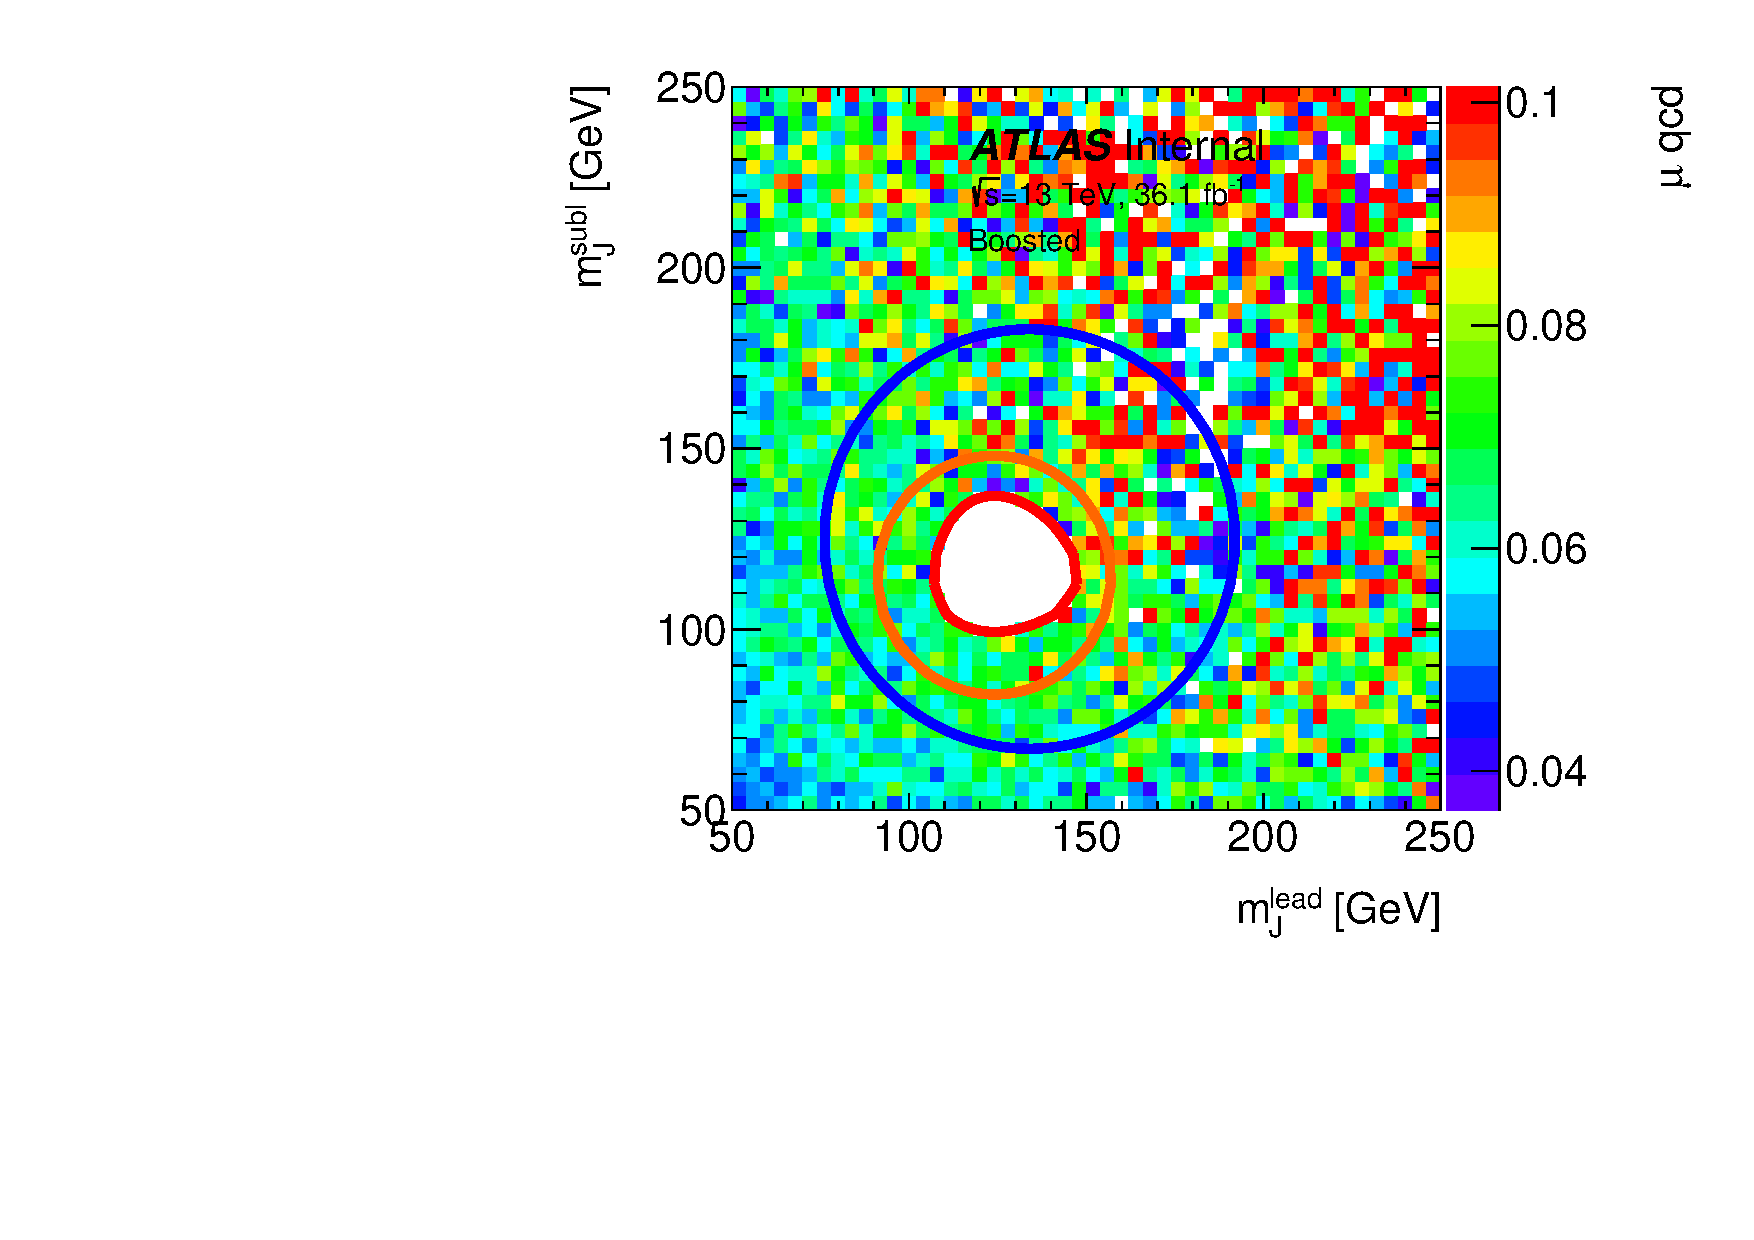
\includegraphics[width=0.45\textwidth,angle=-90]{figures/boosted/AppendixMuqcdstudy/TwoTag_split_Incl_mH0H1.pdf}
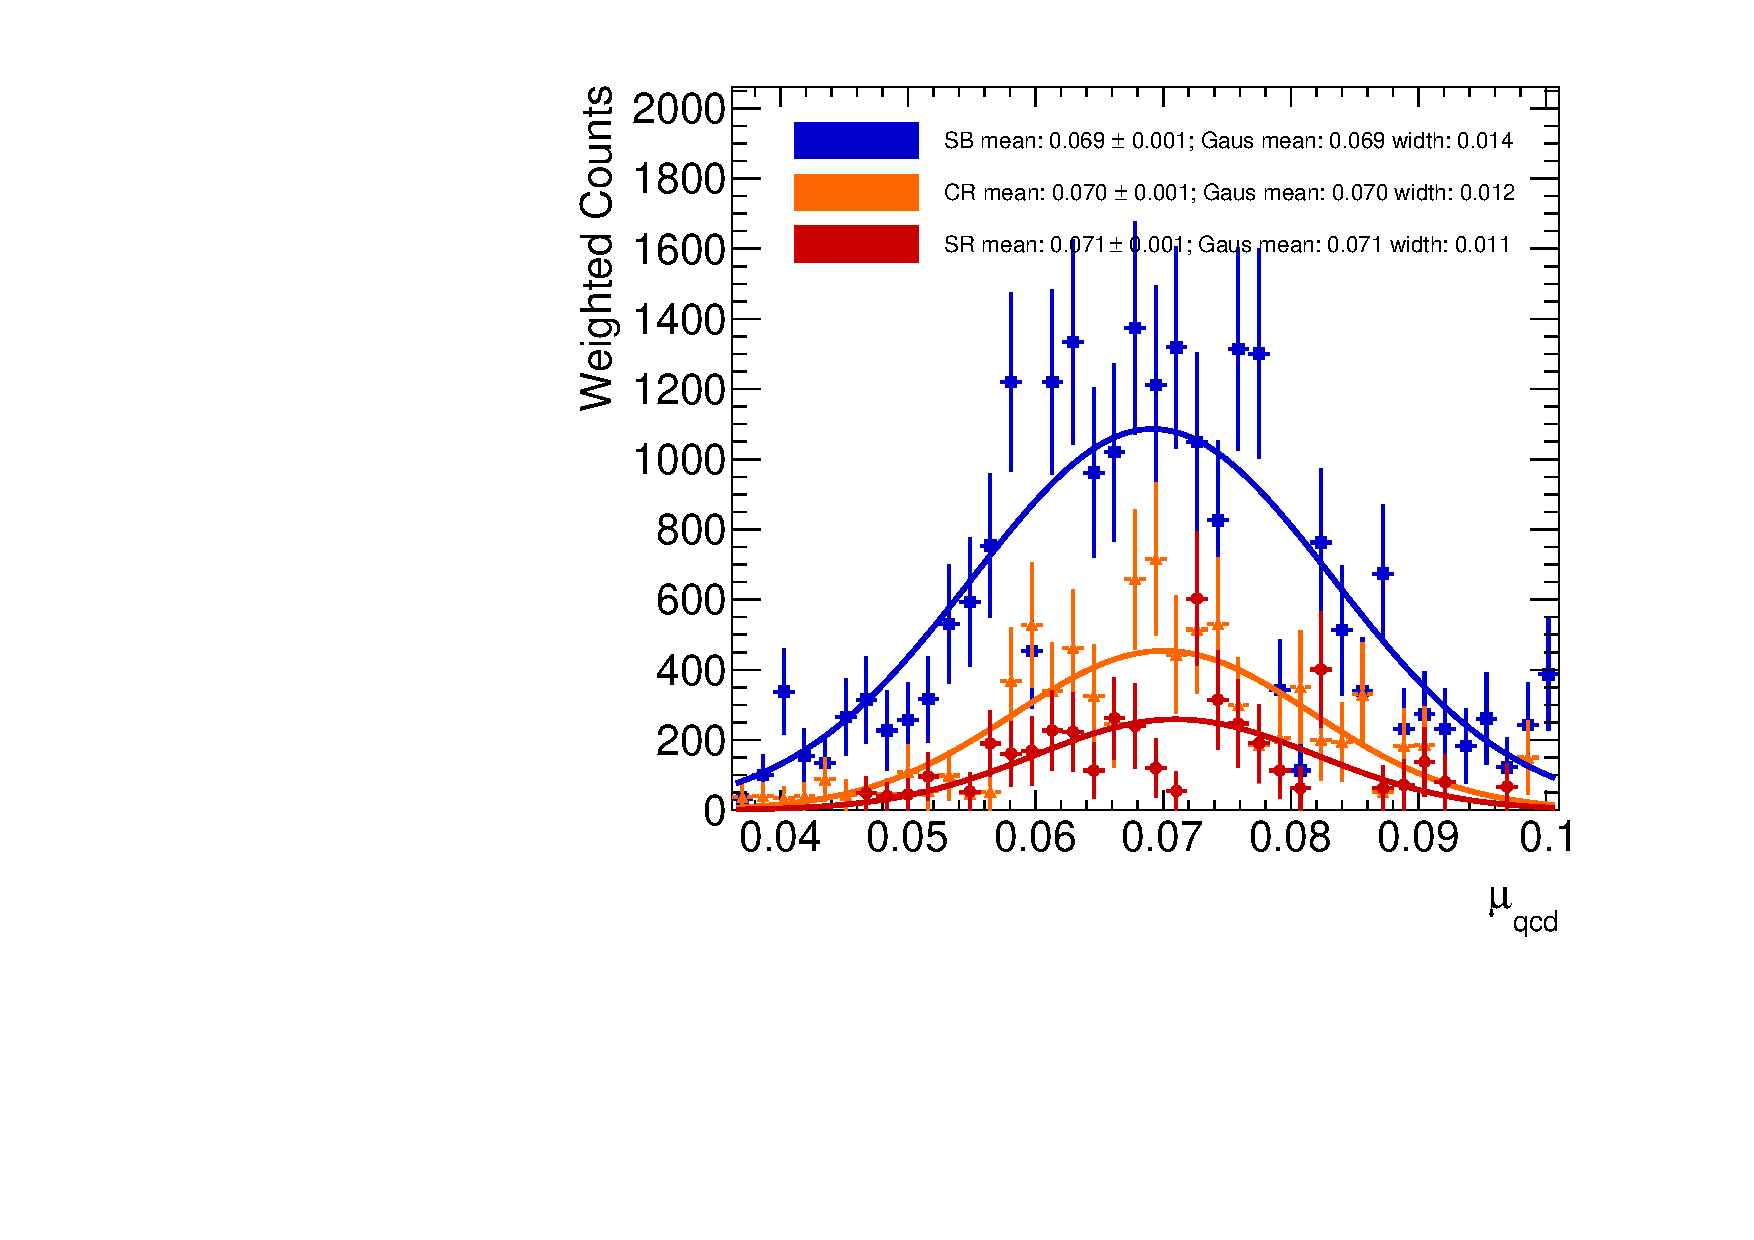
\includegraphics[width=0.45\textwidth,angle=-90]{figures/boosted/AppendixMuqcdstudy/TwoTag_split_Incl_mH0H1_pull.pdf}
\caption{2$b$s over 1$b$ data driven \muqcd values: \muqcd as a funciton of leading Higgs candidate/subleading Higgs candiate mass(left); and \muqcd value pull in Sideband/Control/Signal regions(right), with the weighted mean value and the Guassian fit mean value shown on the plot.}
\label{fig:app-muqcd-2bs}
\end{center}
\end{figure*}

\begin{figure*}[htbp!]
\begin{center}
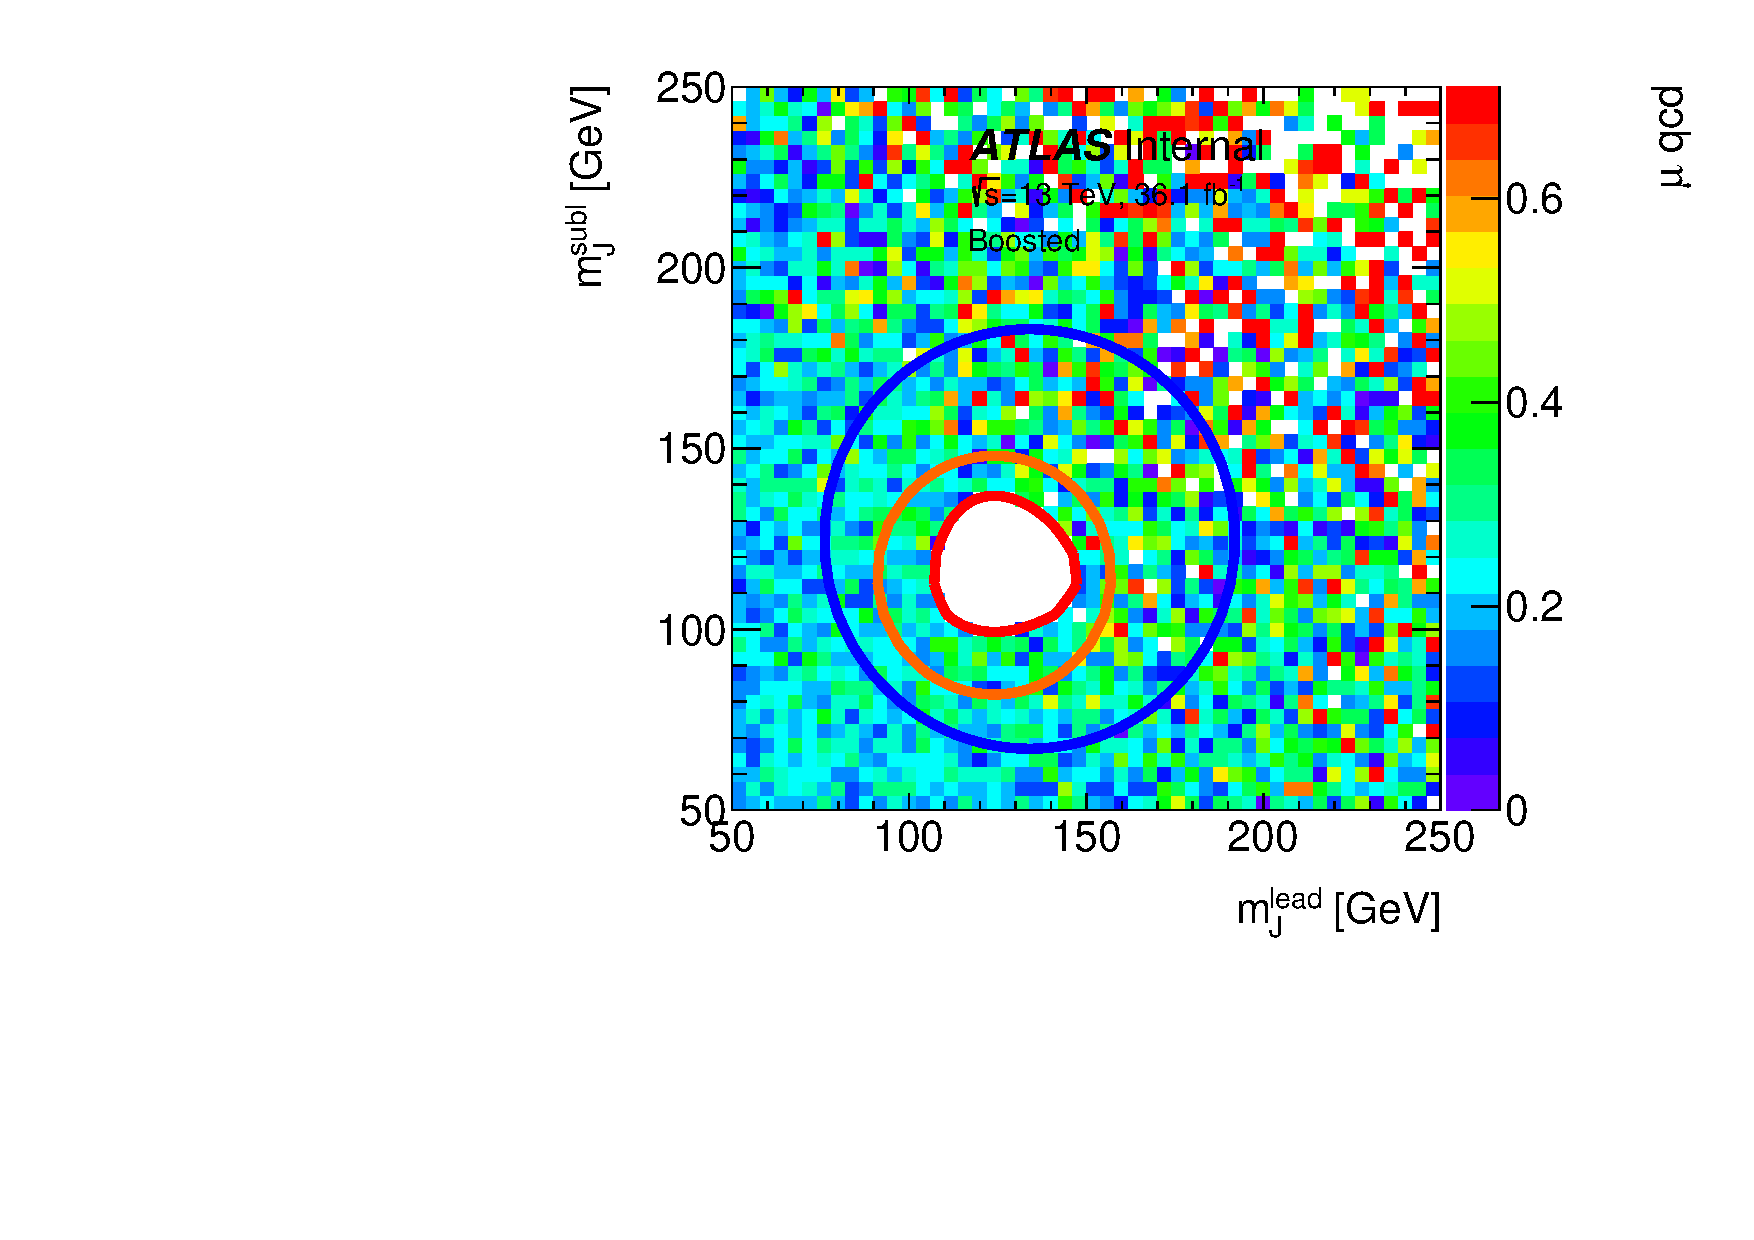
\includegraphics[width=0.45\textwidth,angle=-90]{figures/boosted/AppendixMuqcdstudy/ThreeTag_Incl_mH0H1.pdf}
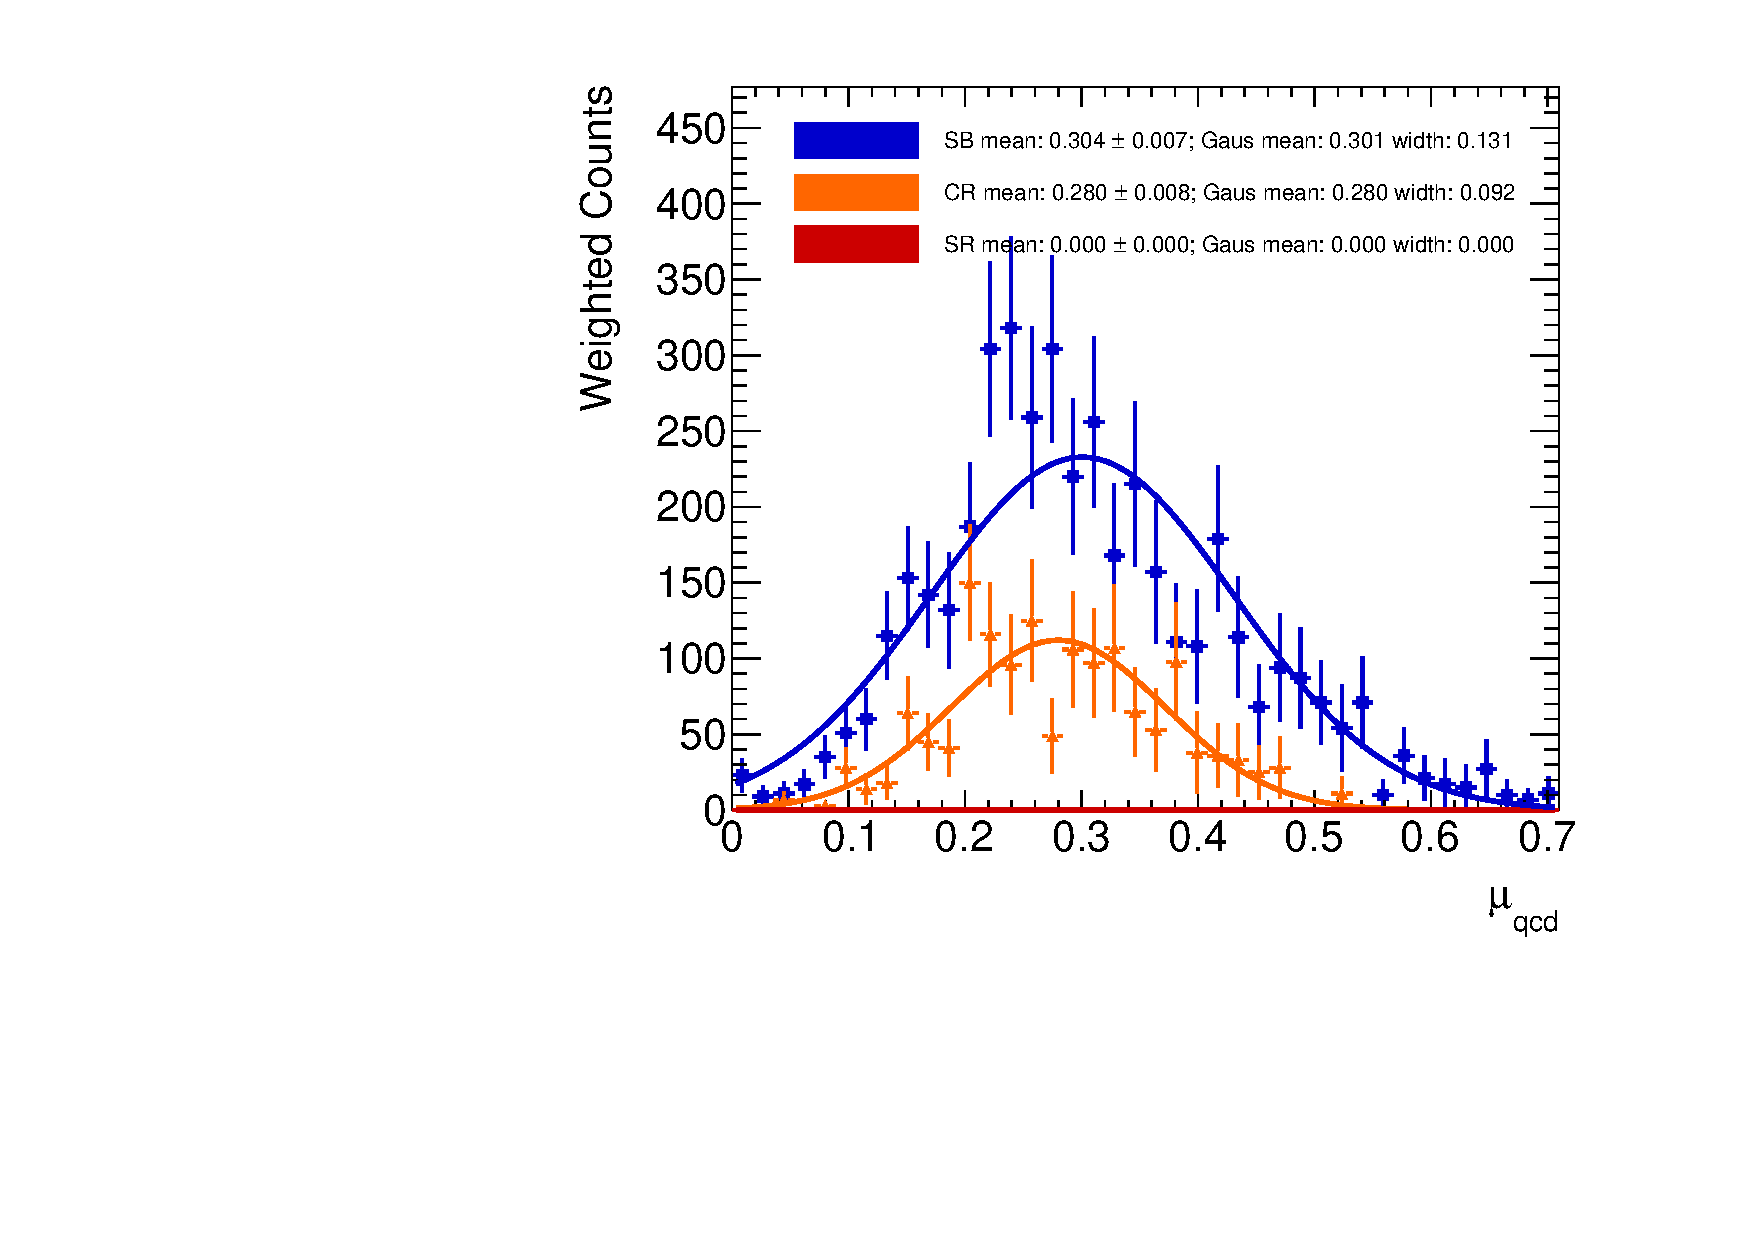
\includegraphics[width=0.45\textwidth,angle=-90]{figures/boosted/AppendixMuqcdstudy/ThreeTag_Incl_mH0H1_pull.pdf}
\caption{3$b$ over 2$b$ data driven \muqcd values: \muqcd as a funciton of leading Higgs candidate/subleading Higgs candiate mass(left); and \muqcd value pull in Sideband/Control/Signal regions(right), with the weighted mean value and the Guassian fit mean value shown on the plot.}
\label{fig:app-muqcd-3b}
\end{center}
\end{figure*}

\begin{figure*}[htbp!]
\begin{center}
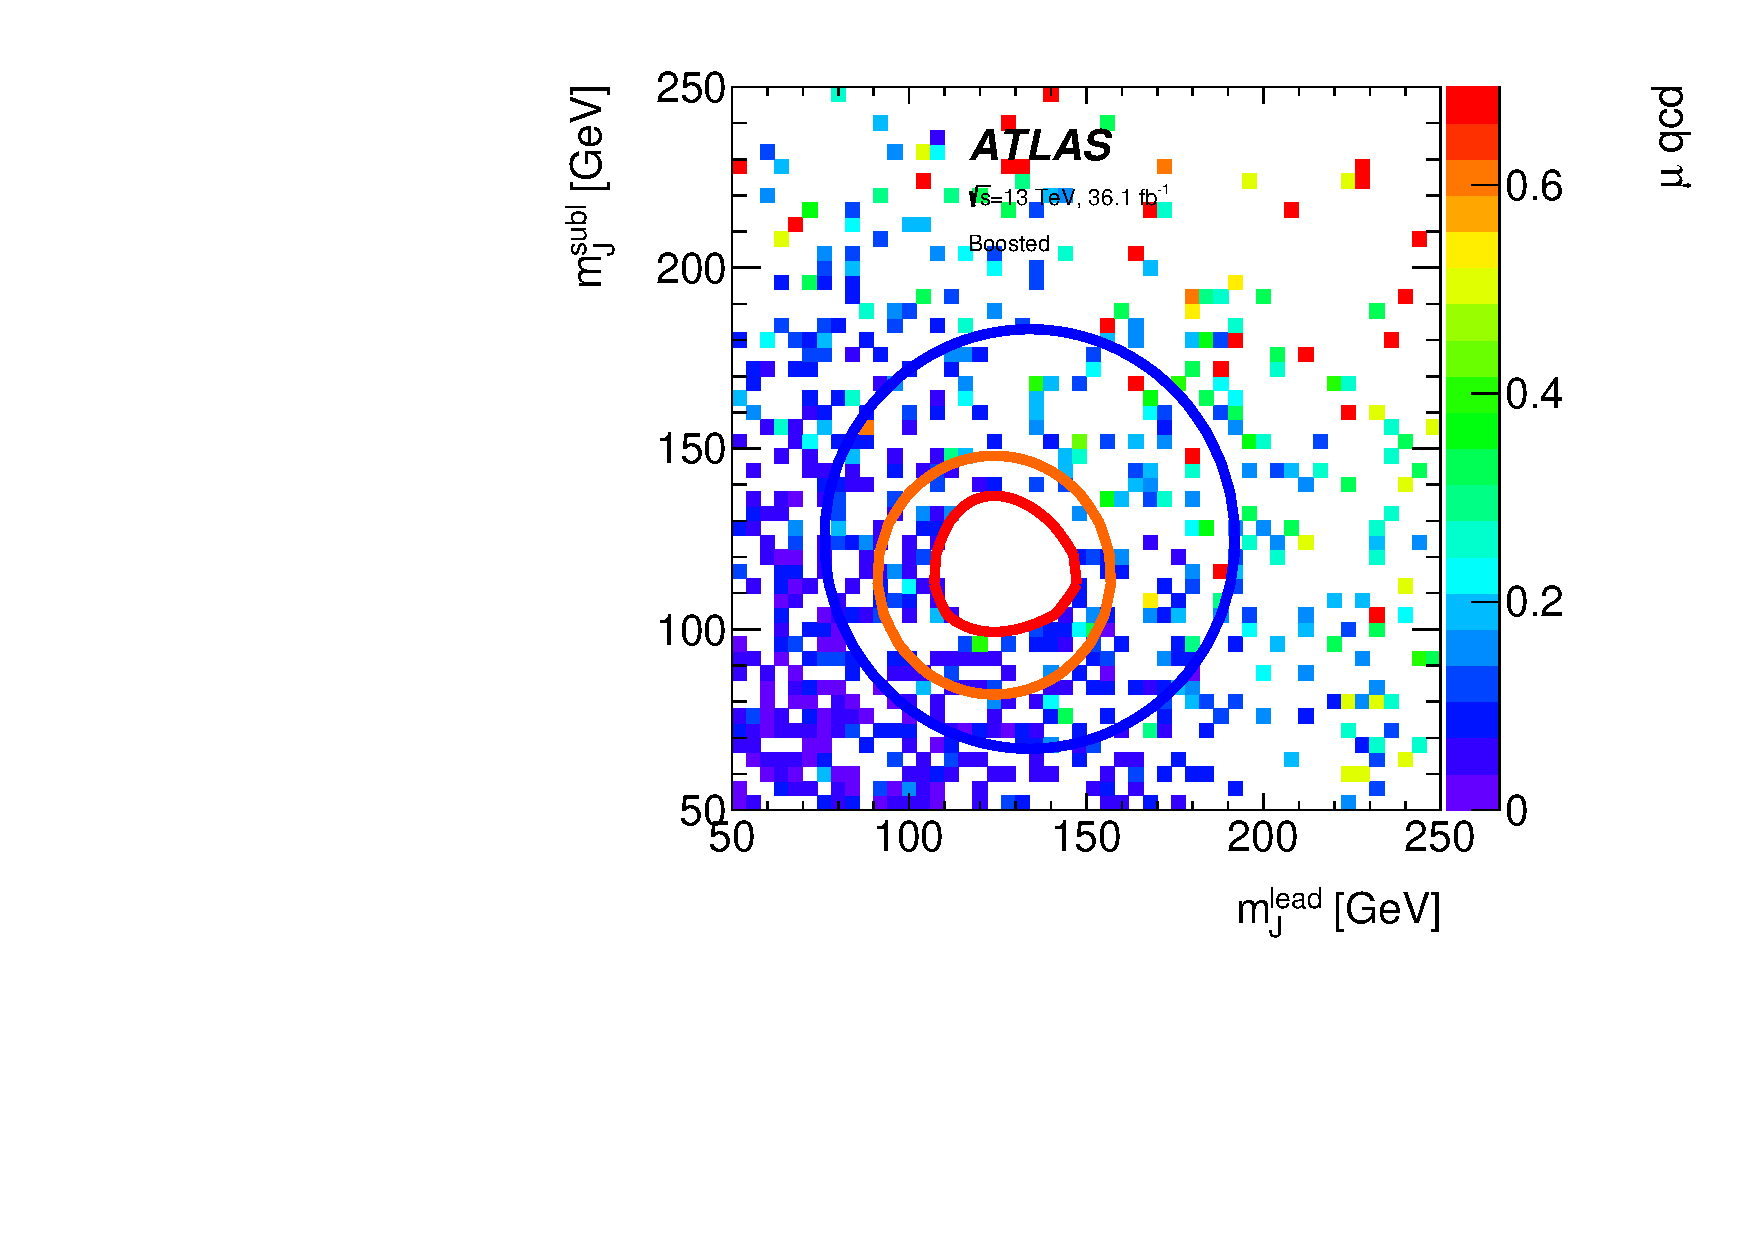
\includegraphics[width=0.45\textwidth,angle=-90]{figures/boosted/AppendixMuqcdstudy/FourTag_Incl_mH0H1.pdf}
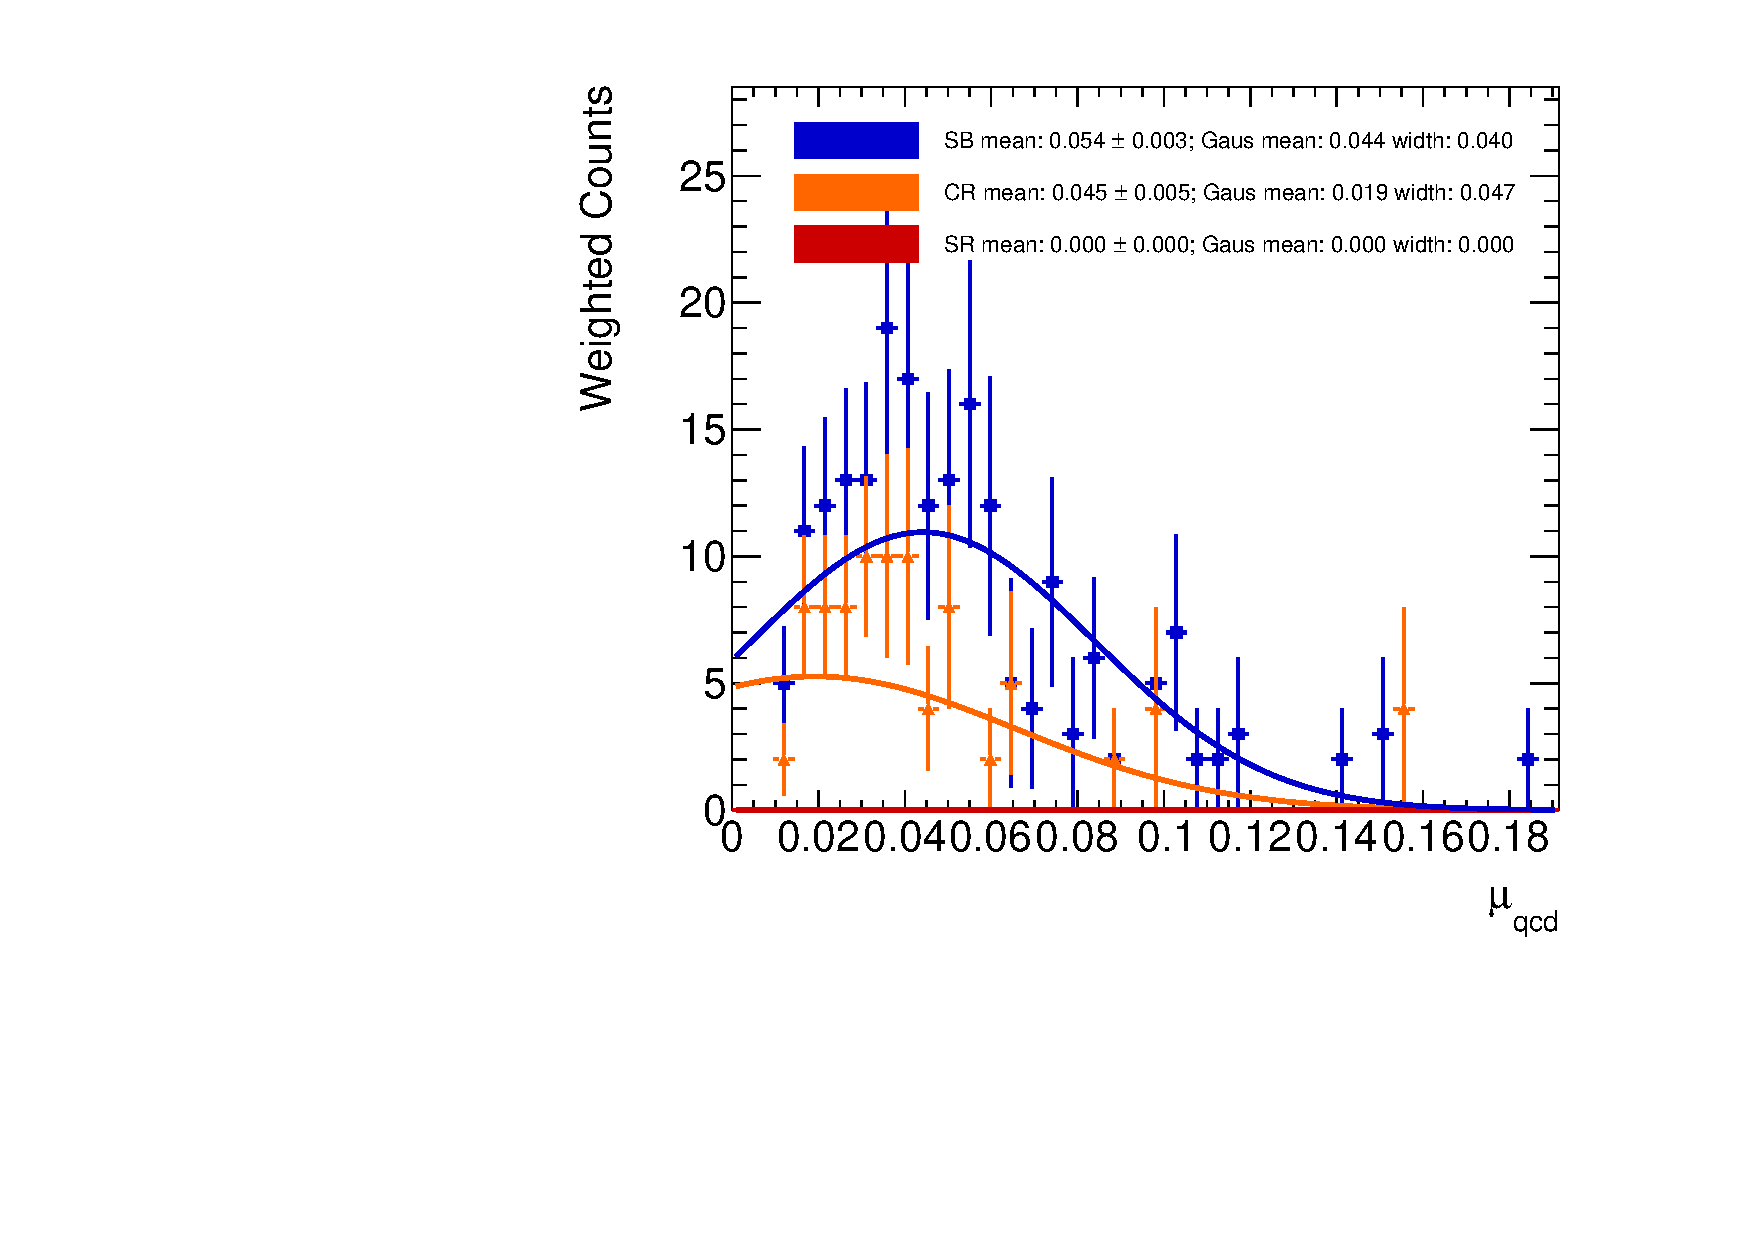
\includegraphics[width=0.45\textwidth,angle=-90]{figures/boosted/AppendixMuqcdstudy/FourTag_Incl_mH0H1_pull.pdf}
\caption{4$b$ over 2$b$ data driven \muqcd values: \muqcd as a funciton of leading Higgs candidate/subleading Higgs candiate mass(left); and \muqcd value pull in Sideband/Control/Signal regions(right), with the weighted mean value and the Guassian fit mean value shown on the plot.}
\label{fig:app-muqcd-4b}
\end{center}
\end{figure*}



\begin{figure*}[htbp!]
\begin{center}
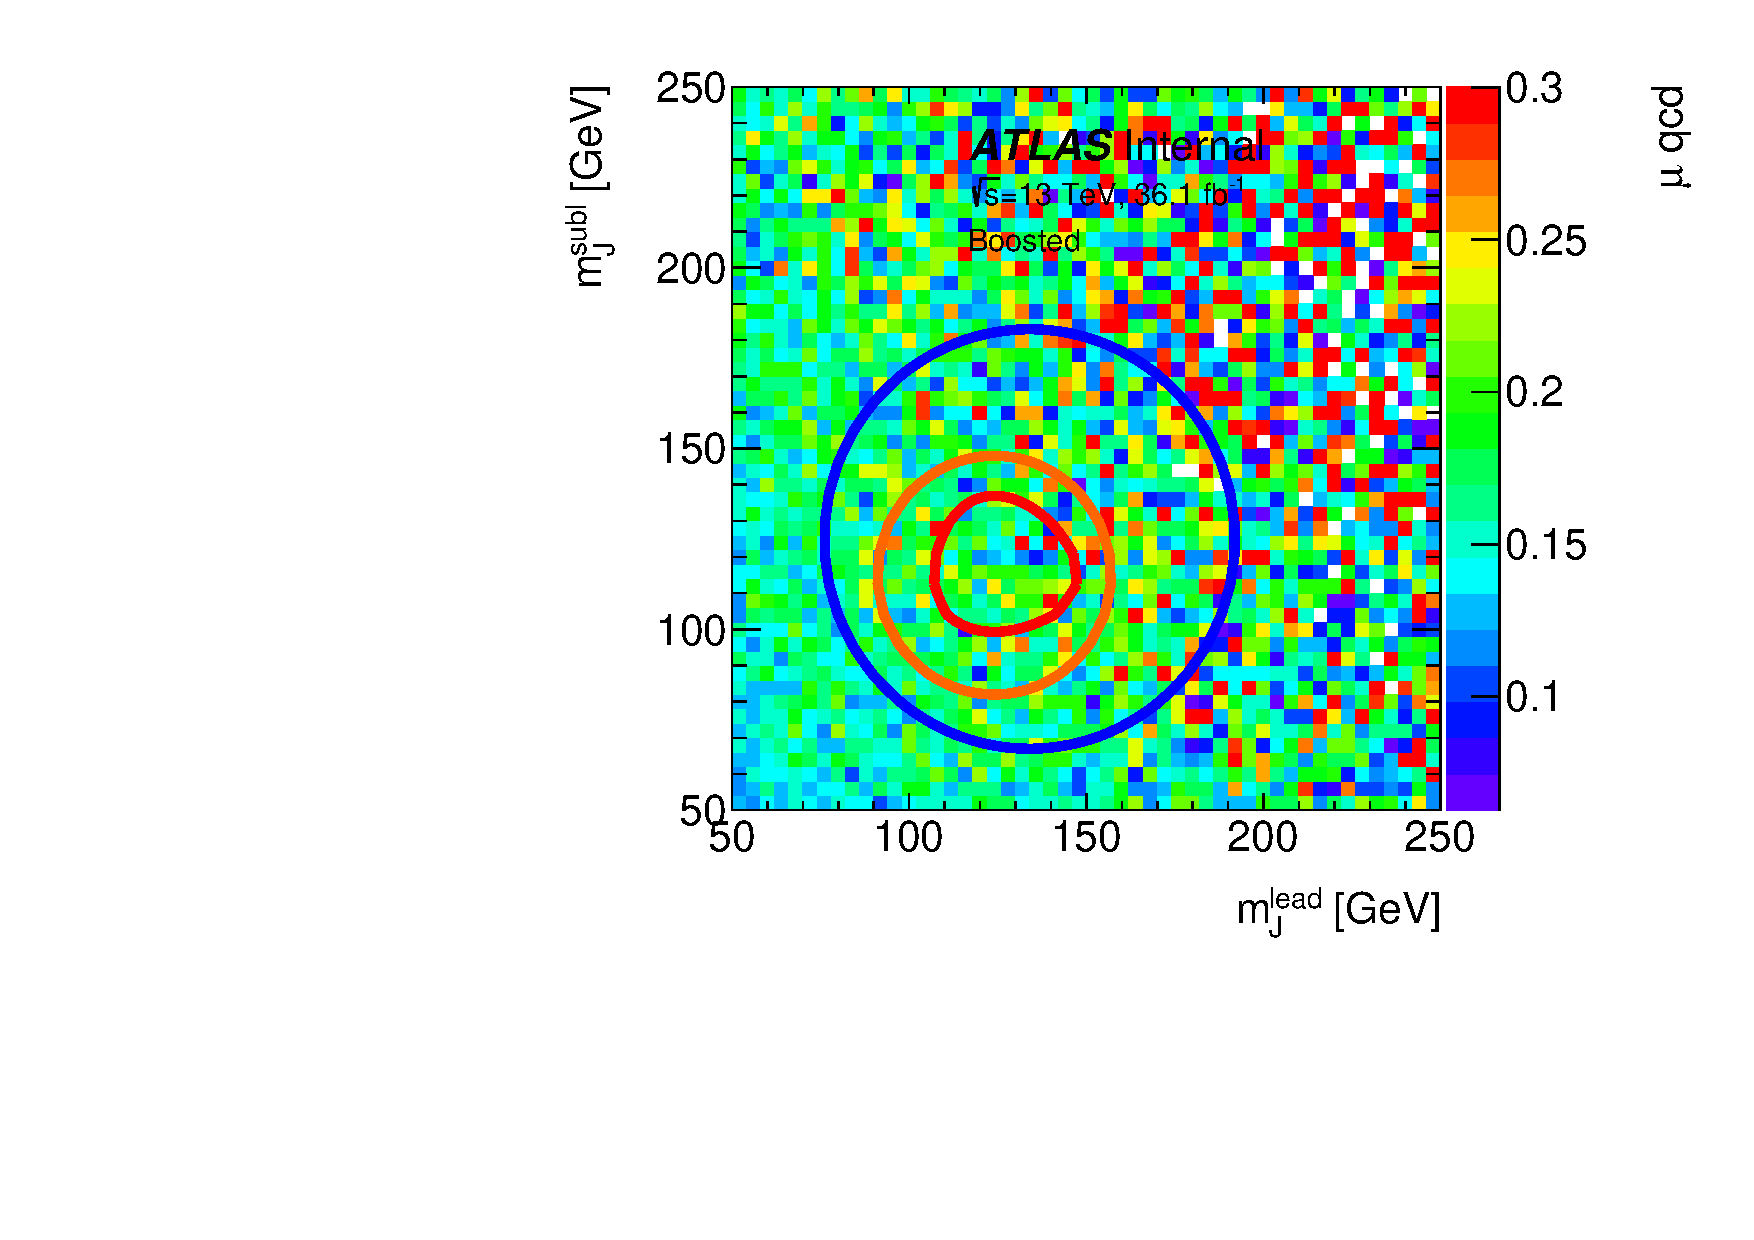
\includegraphics[width=0.45\textwidth,angle=-90]{figures/boosted/AppendixMuqcdstudy/QCD_OneTag_Incl_mH0H1.pdf}
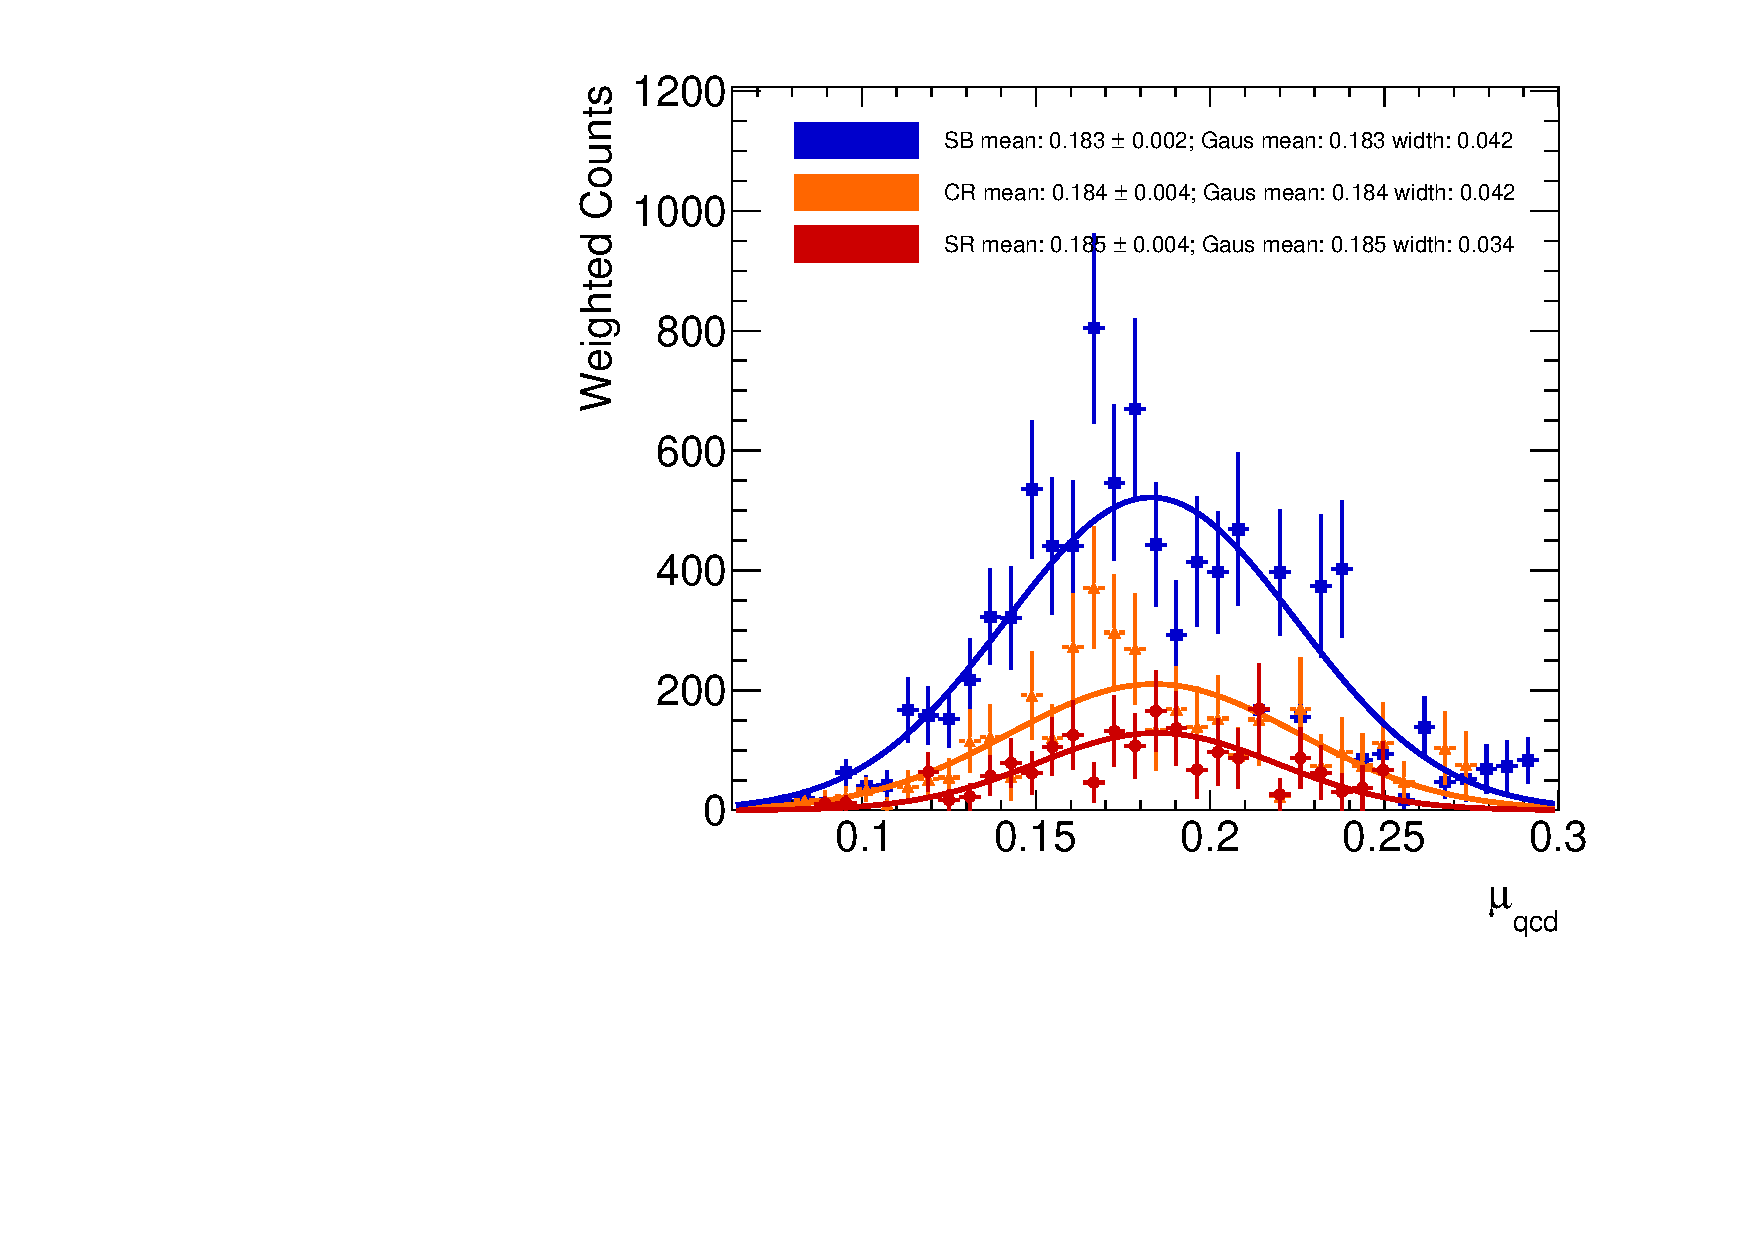
\includegraphics[width=0.45\textwidth,angle=-90]{figures/boosted/AppendixMuqcdstudy/QCD_OneTag_Incl_mH0H1_pull.pdf}
\caption{1$b$ over 0$b$ data driven \muqcd values in dijet MC: \muqcd as a funciton of leading Higgs candidate/subleading Higgs candiate mass(left); and \muqcd value pull in Sideband/Control/Signal regions(right), with the weighted mean value and the Guassian fit mean value shown on the plot.}
\label{fig:app-muqcd-1b-qcd}
\end{center}
\end{figure*}

\begin{figure*}[htbp!]
\begin{center}
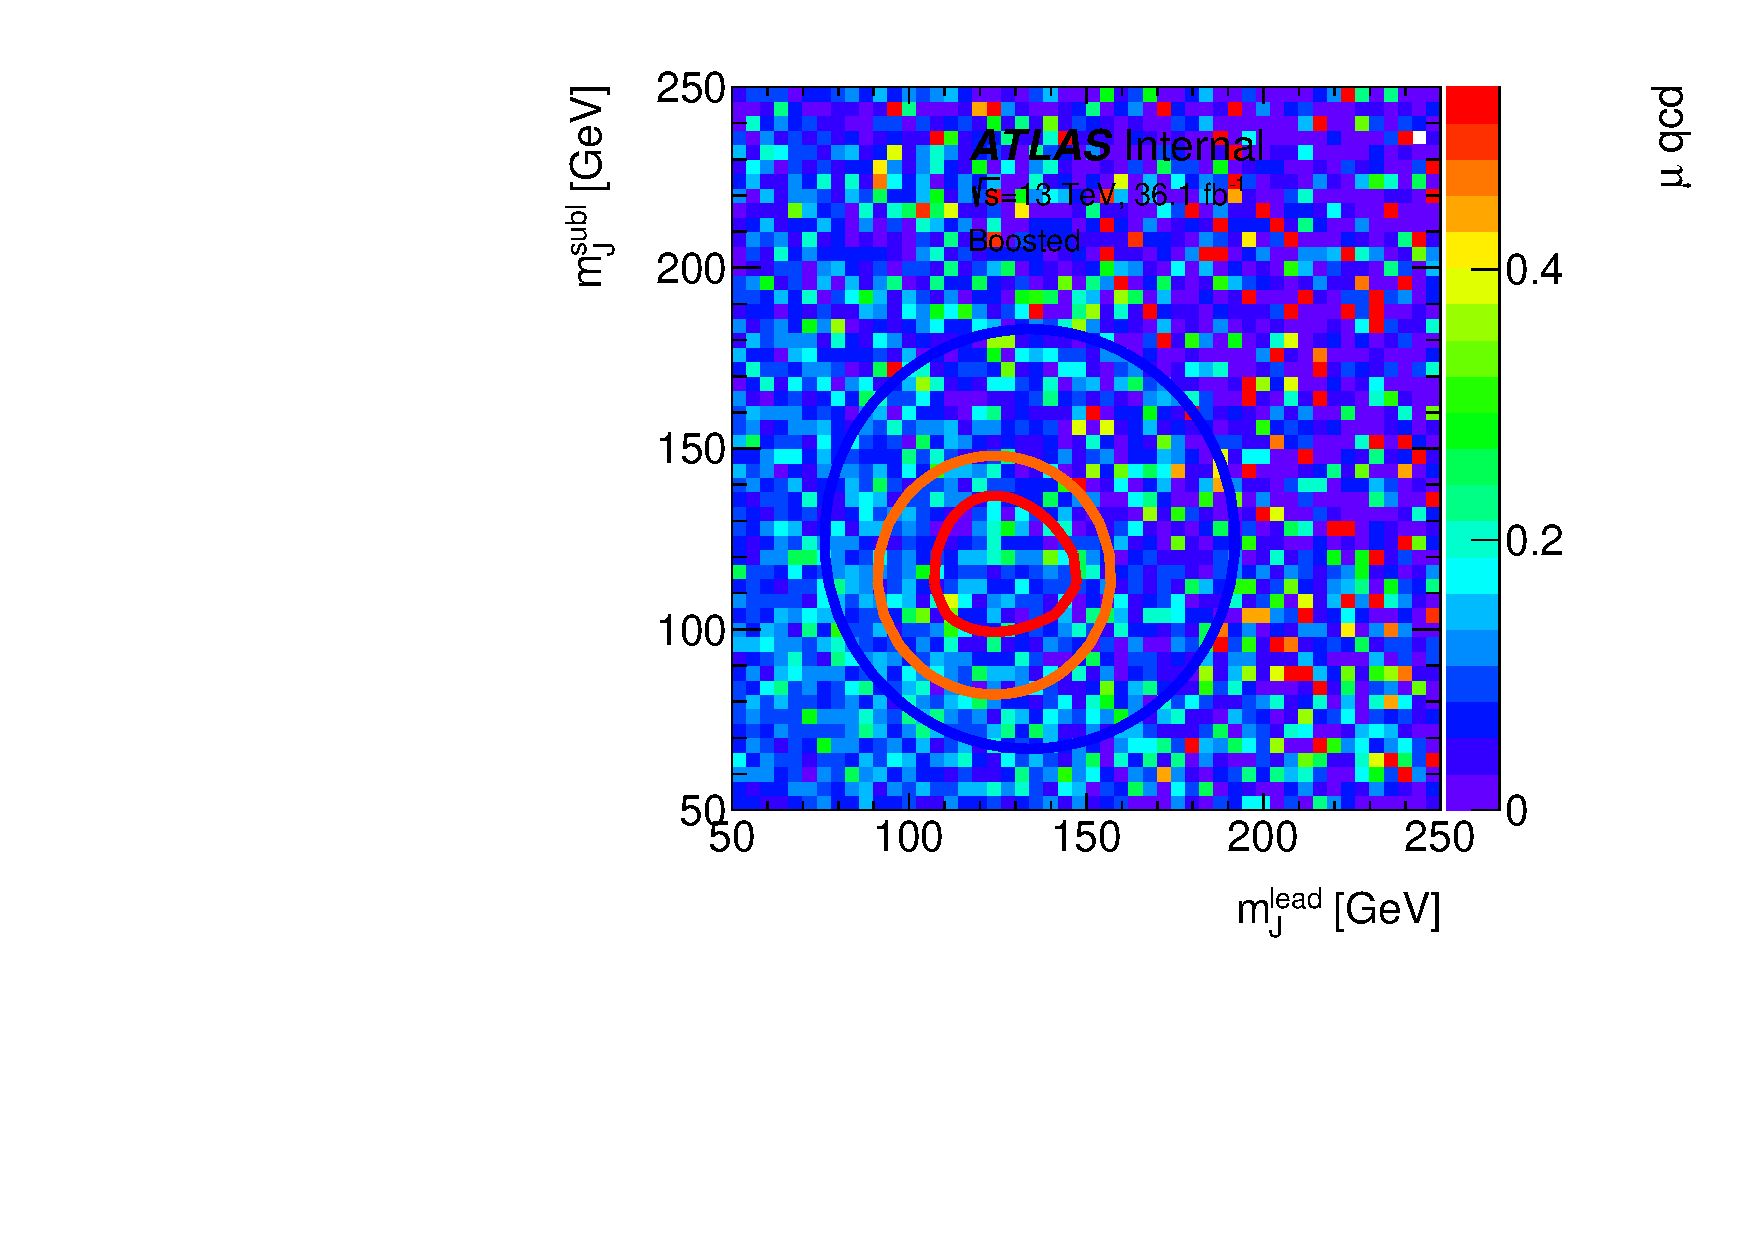
\includegraphics[width=0.45\textwidth,angle=-90]{figures/boosted/AppendixMuqcdstudy/QCD_TwoTag_Incl_mH0H1.pdf}
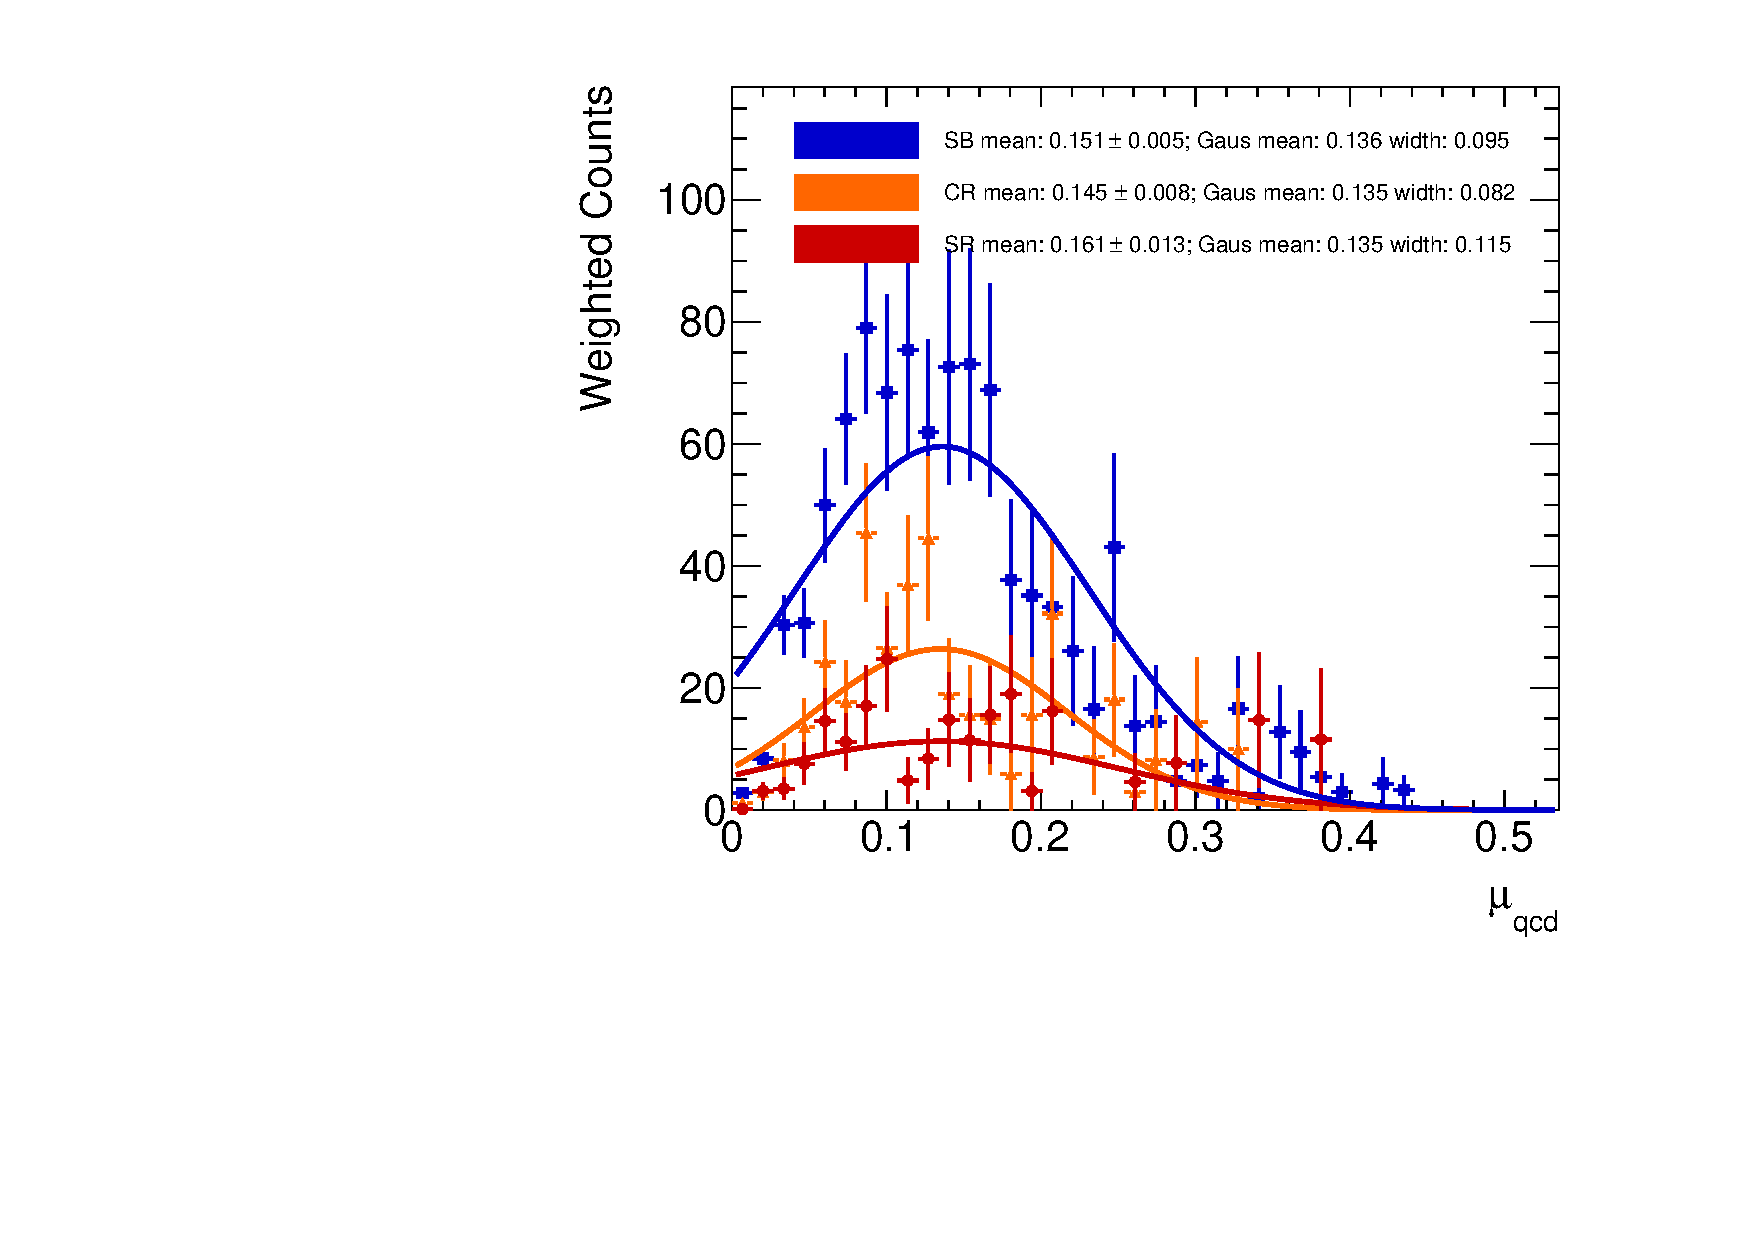
\includegraphics[width=0.45\textwidth,angle=-90]{figures/boosted/AppendixMuqcdstudy/QCD_TwoTag_Incl_mH0H1_pull.pdf}
\caption{2$b$ over 1$b$ data driven \muqcd values in dijet MC: \muqcd as a funciton of leading Higgs candidate/subleading Higgs candiate mass(left); and \muqcd value pull in Sideband/Control/Signal regions(right), with the weighted mean value and the Guassian fit mean value shown on the plot.}
\label{fig:app-muqcd-2b-qcd}
\end{center}
\end{figure*}

\begin{figure*}[htbp!]
\begin{center}
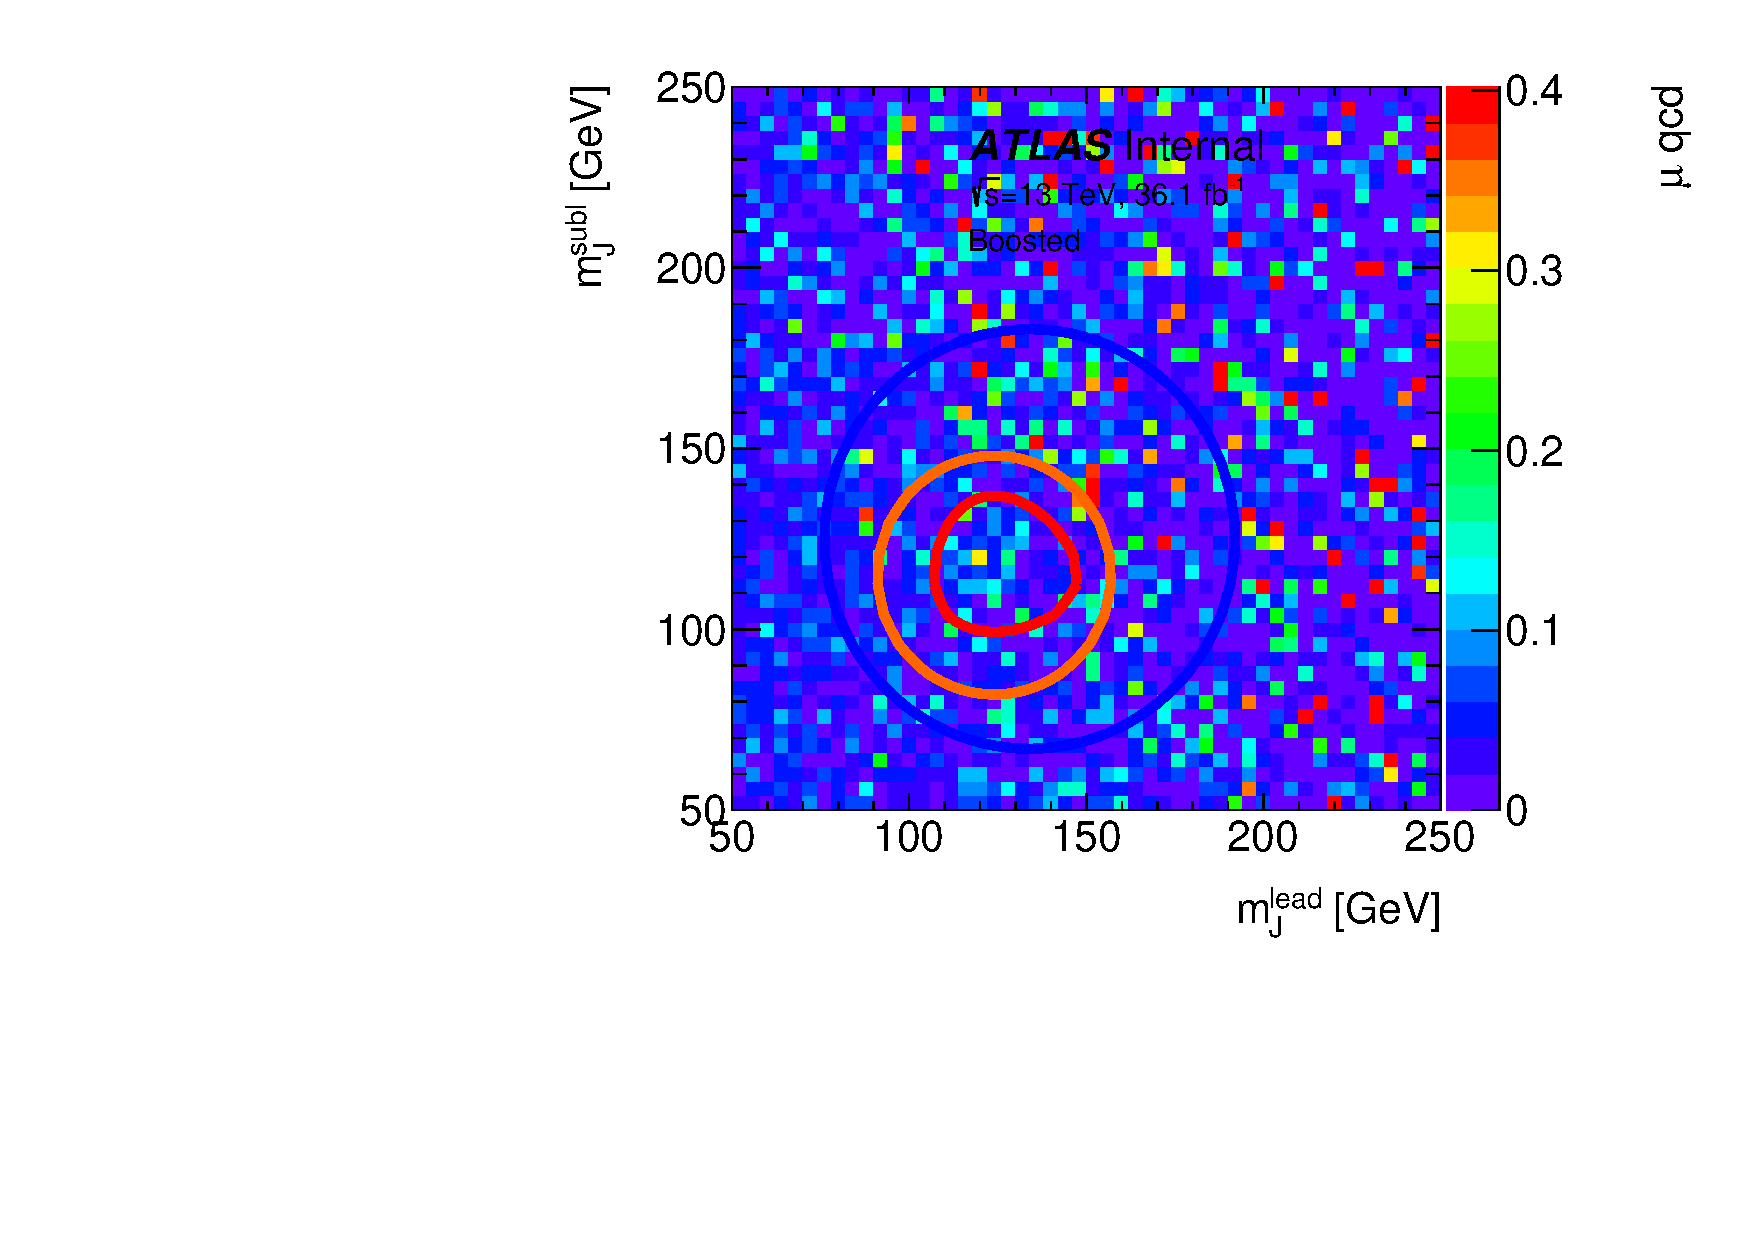
\includegraphics[width=0.45\textwidth,angle=-90]{figures/boosted/AppendixMuqcdstudy/QCD_TwoTag_split_Incl_mH0H1.pdf}
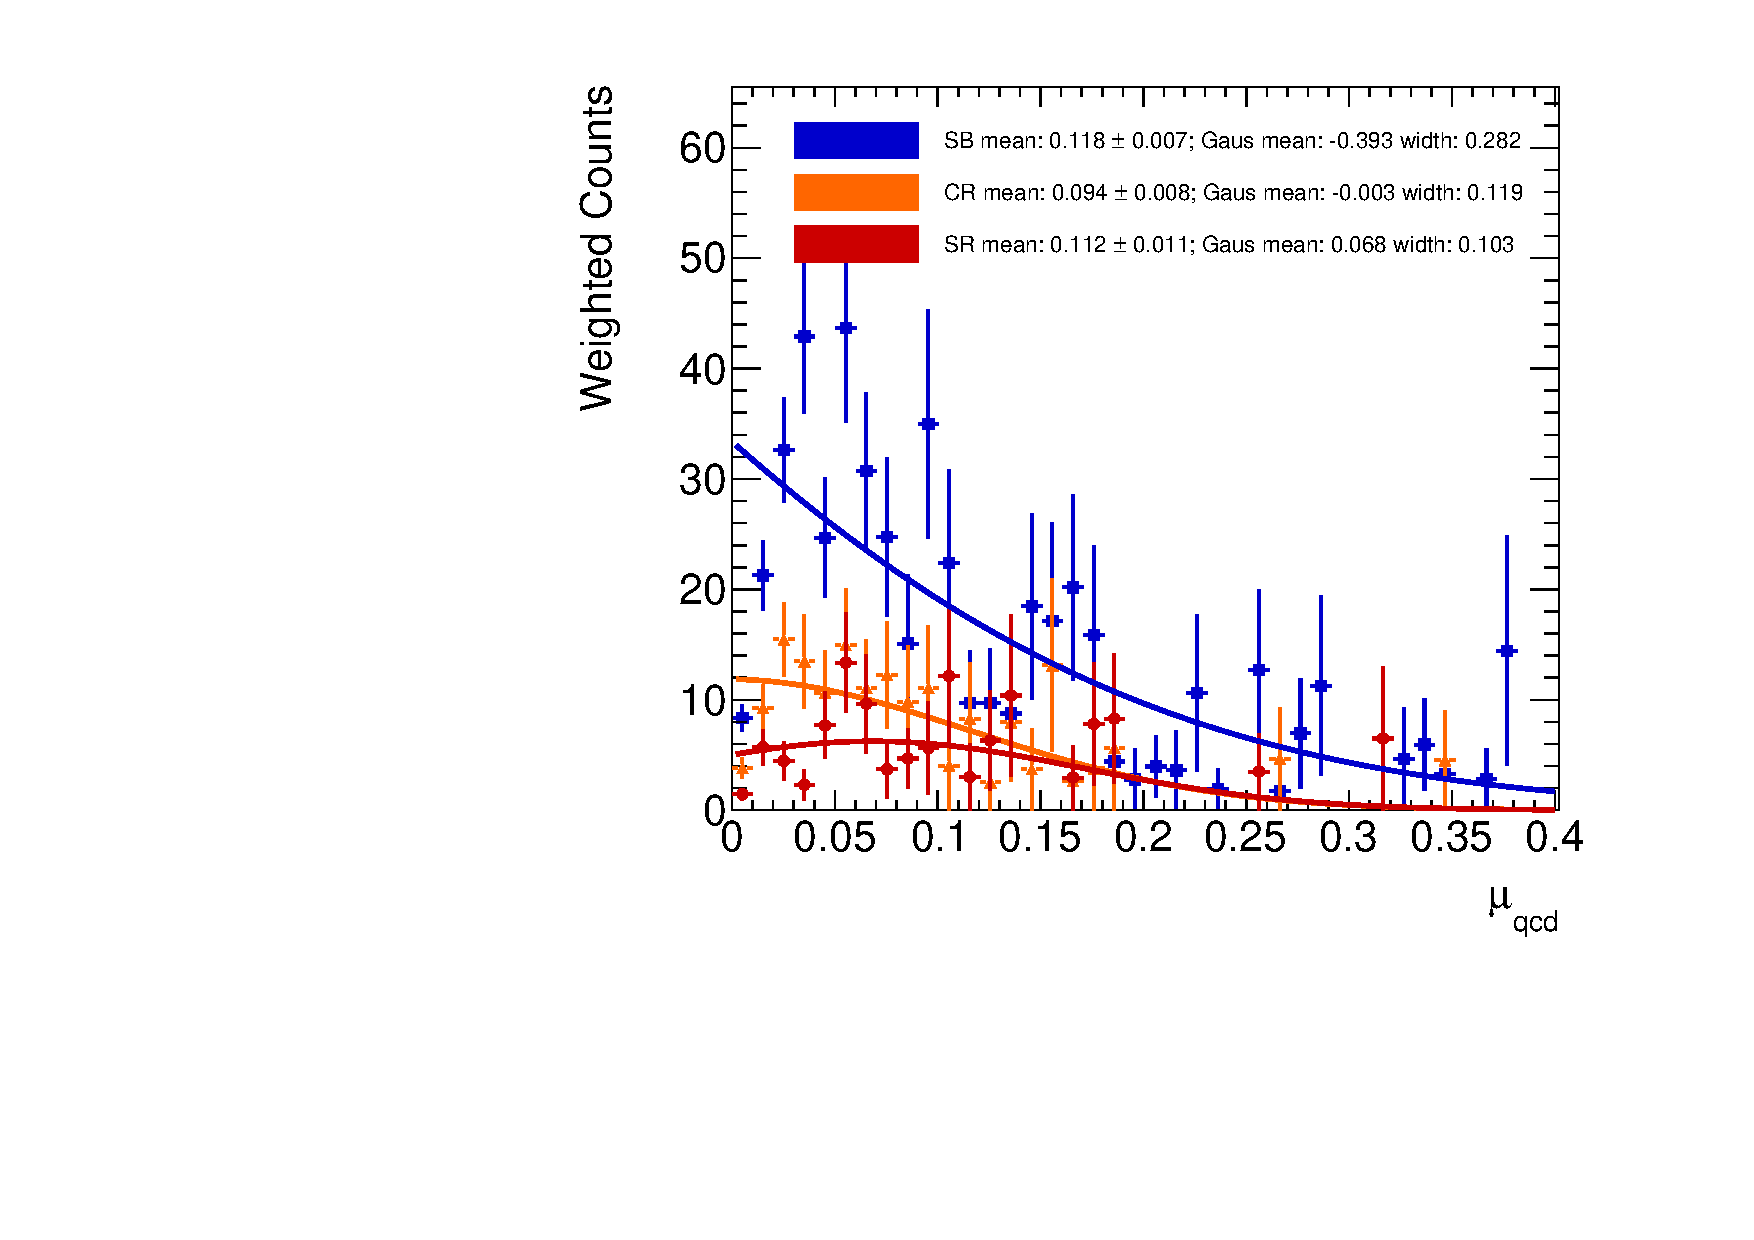
\includegraphics[width=0.45\textwidth,angle=-90]{figures/boosted/AppendixMuqcdstudy/QCD_TwoTag_split_Incl_mH0H1_pull.pdf}
\caption{2$b$s over 1$b$ data driven \muqcd values in dijet MC: \muqcd as a funciton of leading Higgs candidate/subleading Higgs candiate mass(left); and \muqcd value pull in Sideband/Control/Signal regions(right), with the weighted mean value and the Guassian fit mean value shown on the plot. Poor Statistics of the dijet MC affect the pull distributions.}
\label{fig:app-muqcd-2bs-qcd}
\end{center}
\end{figure*}

\begin{figure*}[htbp!]
\begin{center}
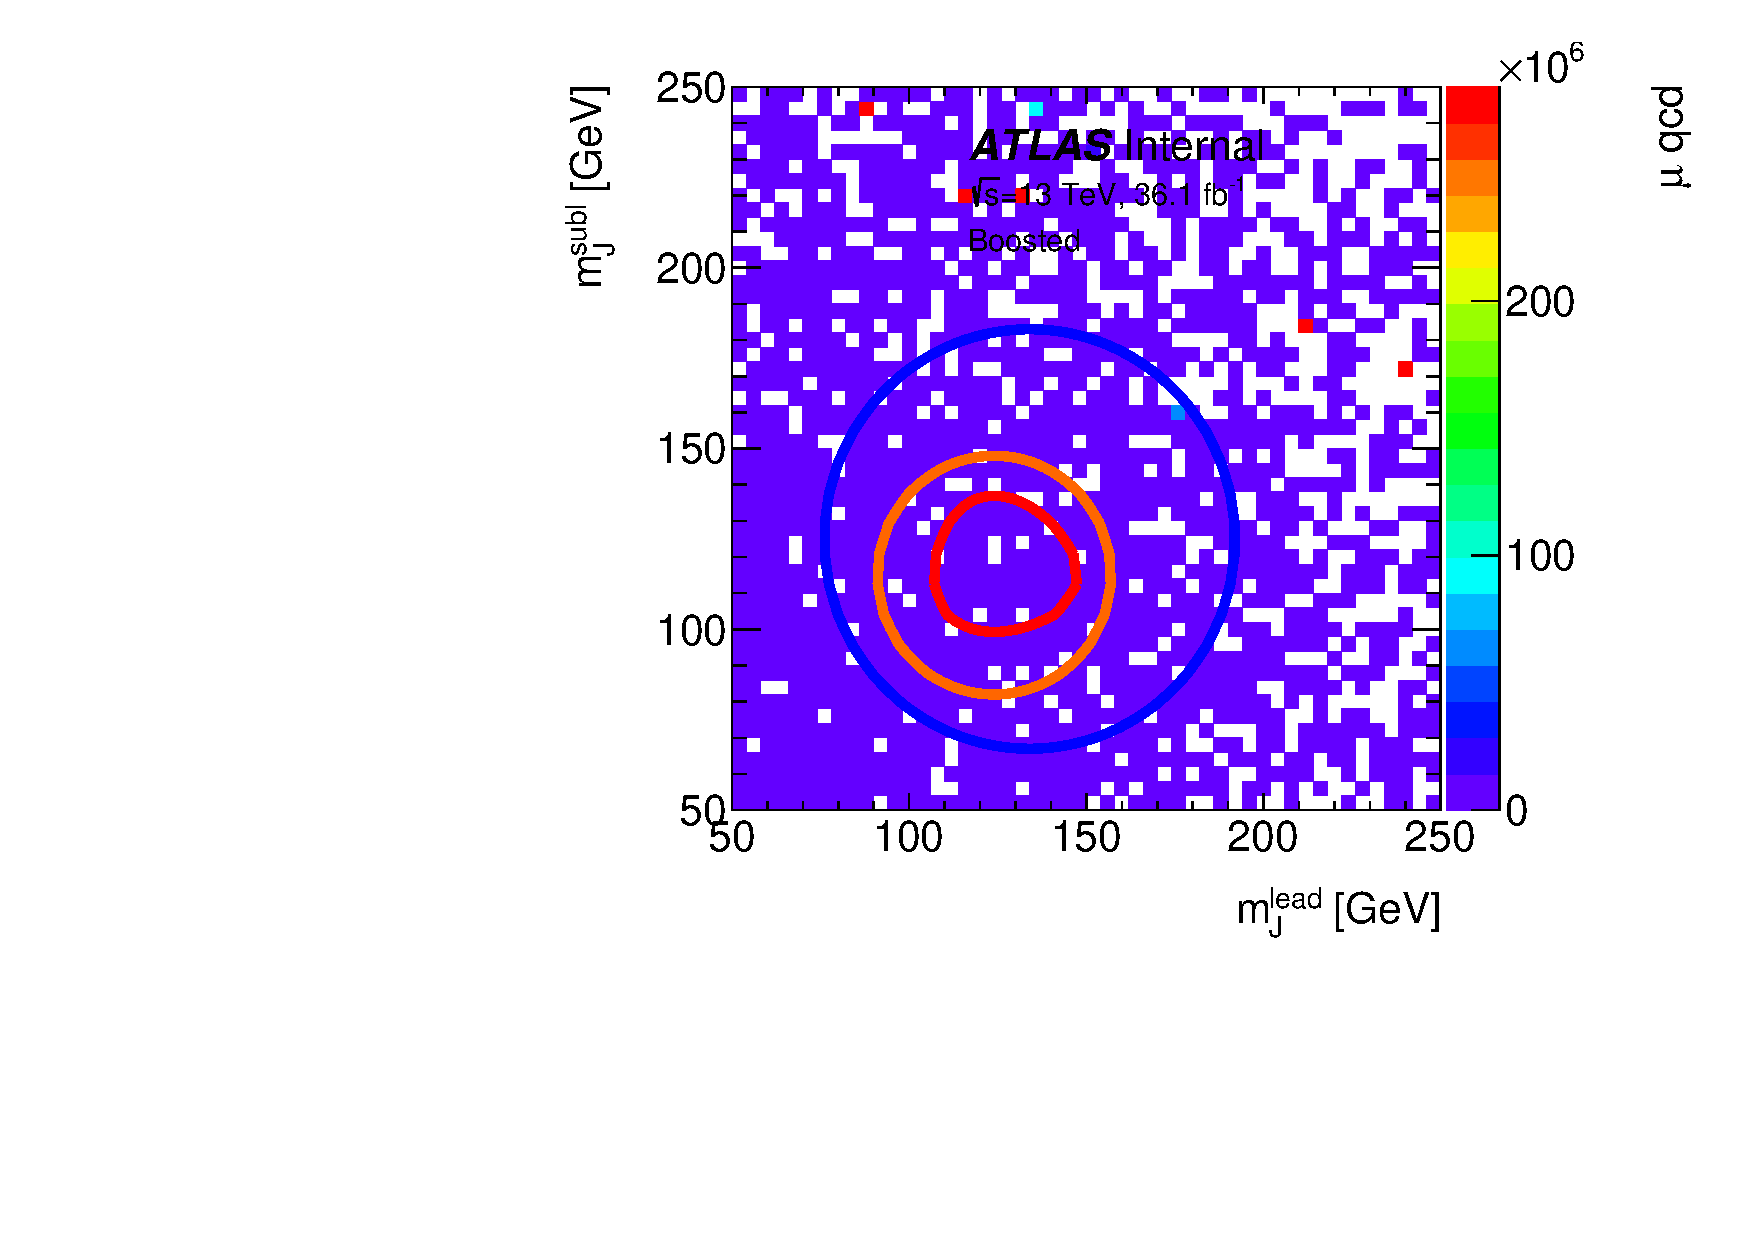
\includegraphics[width=0.45\textwidth,angle=-90]{figures/boosted/AppendixMuqcdstudy/QCD_ThreeTag_Incl_mH0H1.pdf}
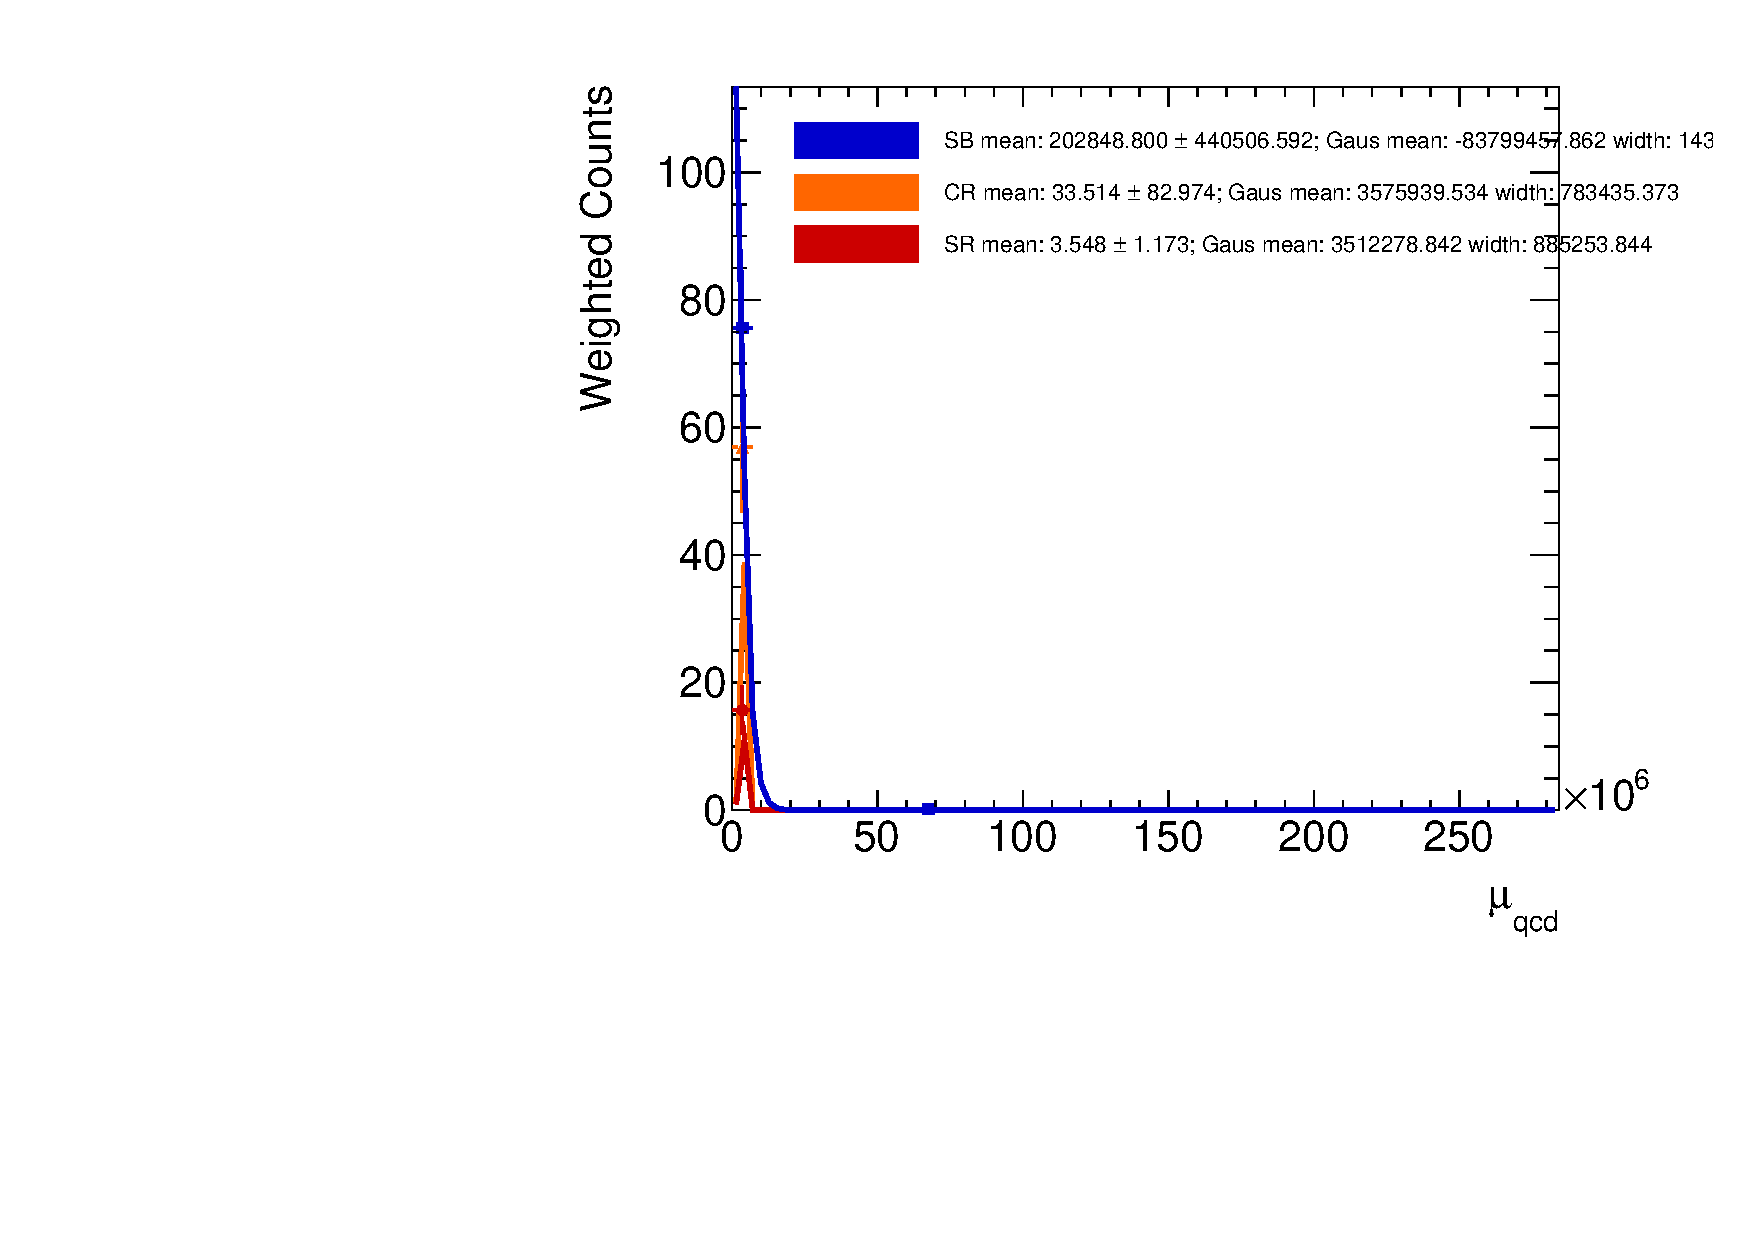
\includegraphics[width=0.45\textwidth,angle=-90]{figures/boosted/AppendixMuqcdstudy/QCD_ThreeTag_Incl_mH0H1_pull.pdf}
\caption{3$b$ over 2$b$ data driven \muqcd values in dijet MC: \muqcd as a funciton of leading Higgs candidate/subleading Higgs candiate mass(left); and \muqcd value pull in Sideband/Control/Signal regions(right), with the weighted mean value and the Guassian fit mean value shown on the plot. Poor Statistics of the dijet MC affect the pull distributions.}
\label{fig:app-muqcd-3b-qcd}
\end{center}
\end{figure*}

\begin{figure*}[htbp!]
\begin{center}
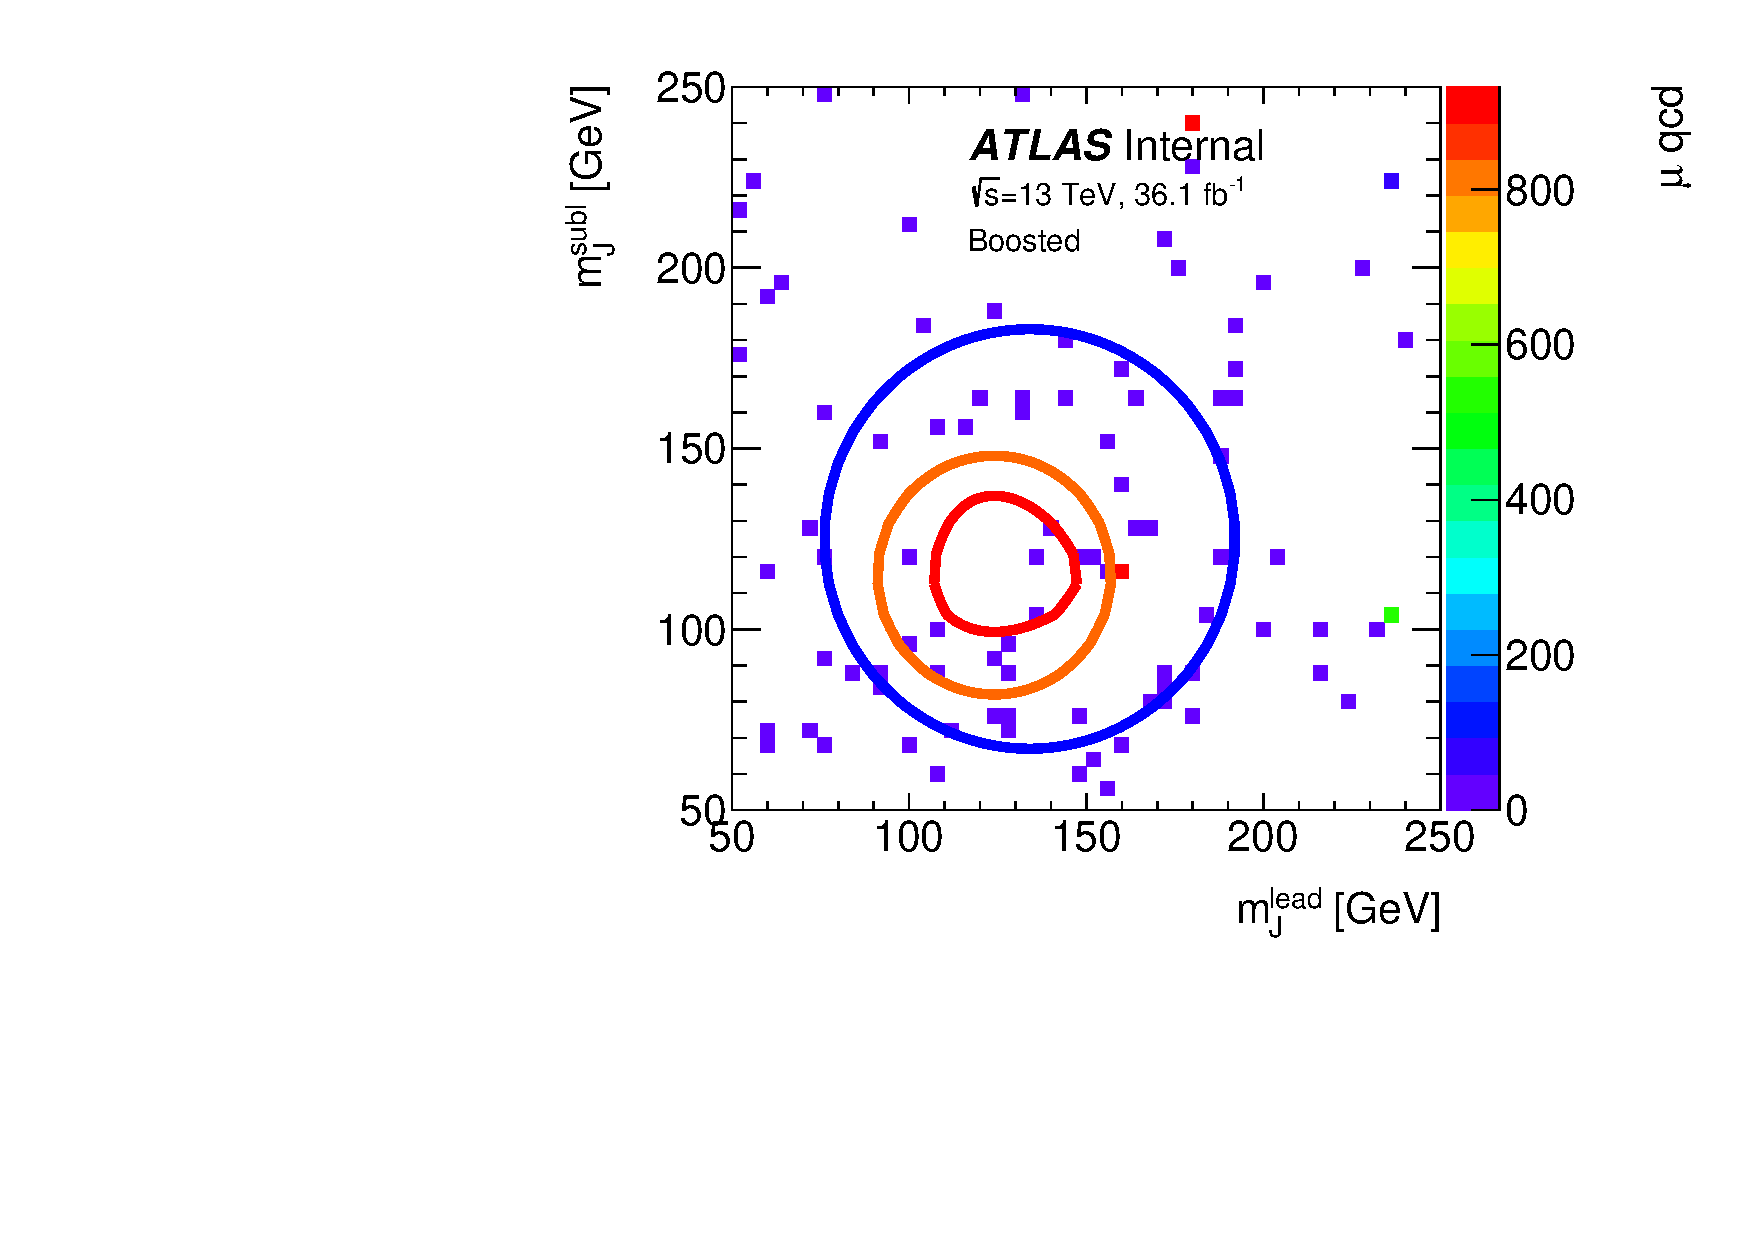
\includegraphics[width=0.45\textwidth,angle=-90]{figures/boosted/AppendixMuqcdstudy/QCD_FourTag_Incl_mH0H1.pdf}
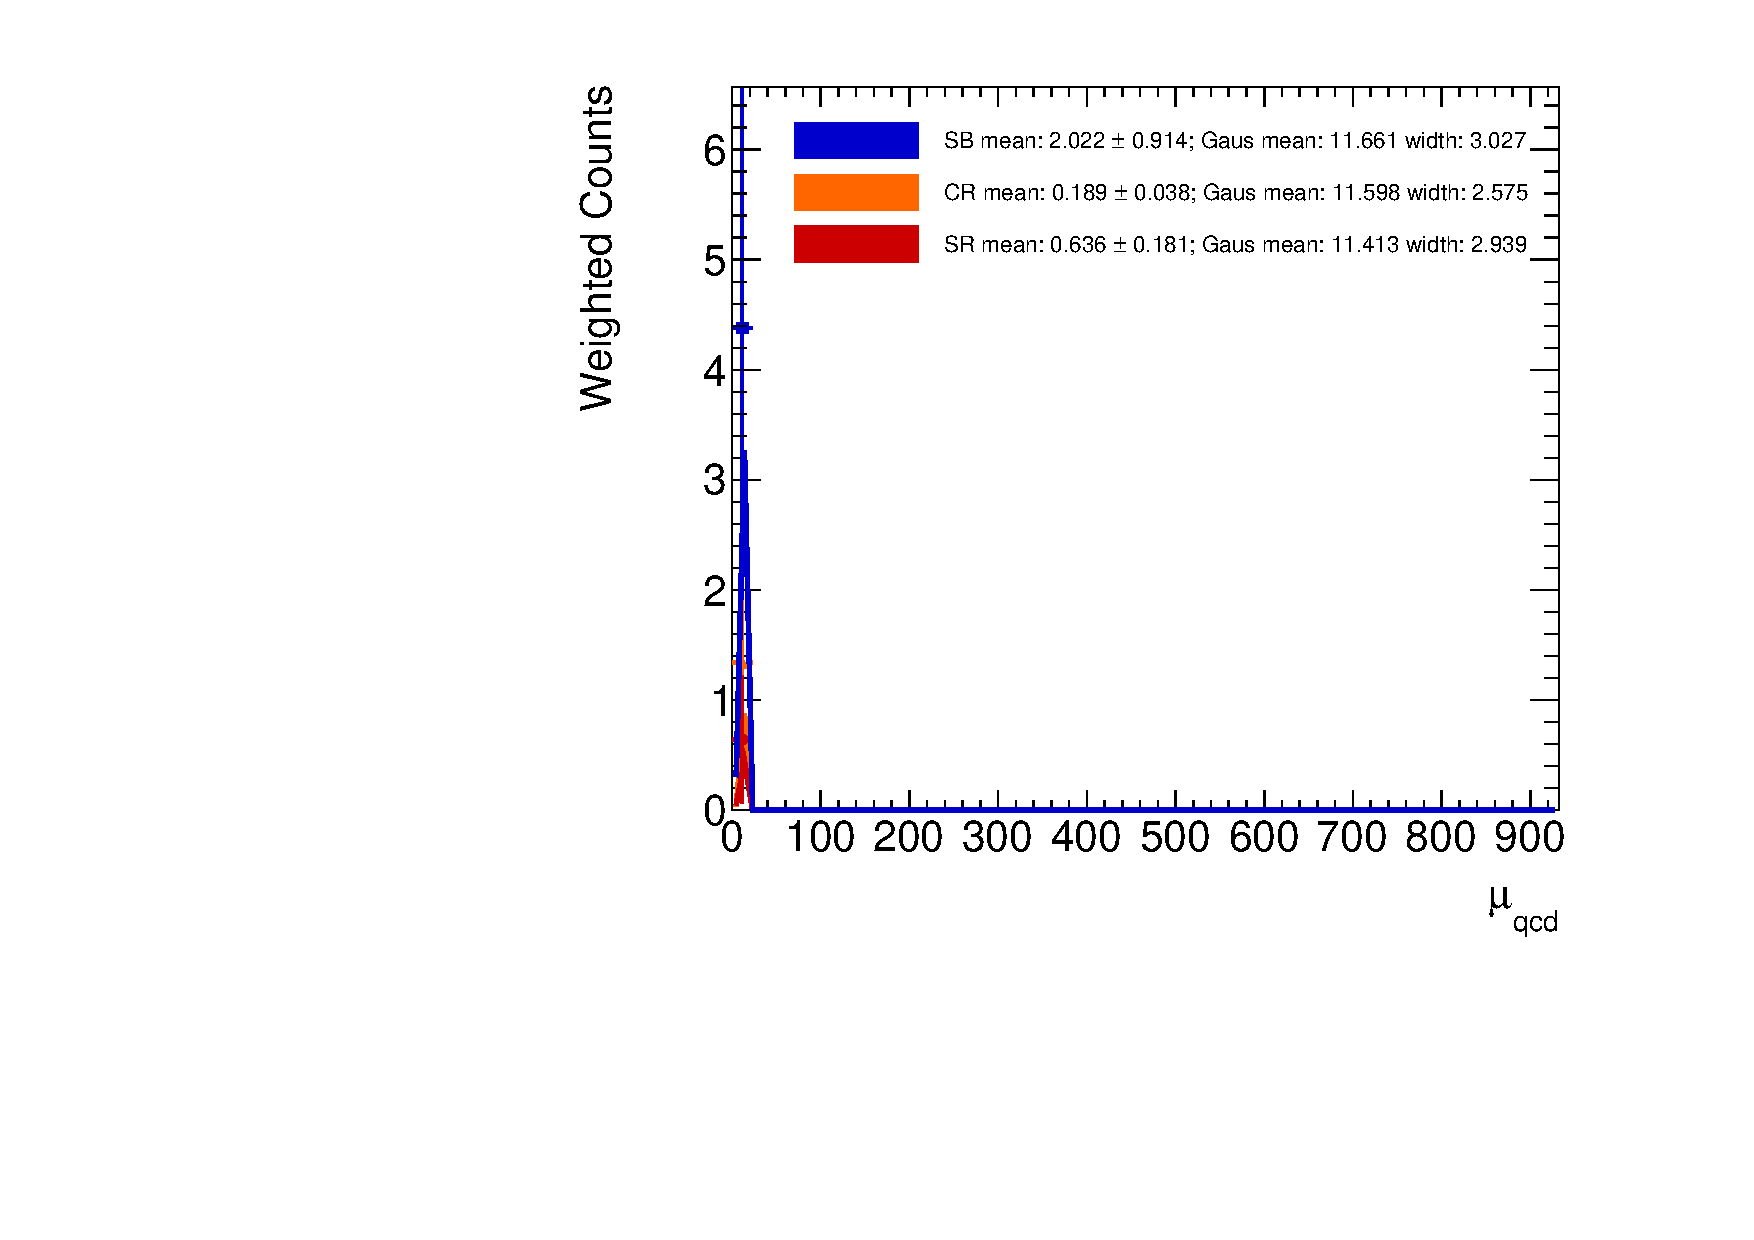
\includegraphics[width=0.45\textwidth,angle=-90]{figures/boosted/AppendixMuqcdstudy/QCD_FourTag_Incl_mH0H1_pull.pdf}
\caption{4$b$ over 2$b$ data driven \muqcd values in dijet MC: \muqcd as a funciton of leading Higgs candidate/subleading Higgs candiate mass(left); and \muqcd value pull in Sideband/Control/Signal regions(right), with the weighted mean value and the Guassian fit mean value shown on the plot. Poor Statistics of the dijet MC affect the pull distributions.}
\label{fig:app-muqcd-4b-qcd}
\end{center}
\end{figure*}

% %%\paragraph{}
% Dijet QCD MC are used to validate the method. We process the Dijet MC using normal event selections, and then add in $t\bar{t}$ and $Z$+jets MC samples to create a "fake" data set, where everything comes from simulations. Then, we proceed the normal analysis steps, subtract the $t\bar{t}$ and $Z$+jets contributions, and obtain the 0$b$ Tag Sideband, Control and Signal region predictions. Then we can use the usual estimation method to gain an $\mu_{qcd}$ estimation for 1$b$, 2$b$, 2$b$s, 3$b$ and 4$b$, since in this way, $\mu_{qcd ntag} = \frac{N_{N Tag SB}}{N_{0 Tag SB}}$. We can also compare the method before and after the fit on leading jet mass is performed. The fit parameters are shown in table  ~\ref{tab:muqcd-fitparameter}. The result is shown in table ~\ref{tab:muqcd-cutflow}.

% \begin{table}[htbp!]
% \begin{center}
% %\input{figures/tables/normfit_mutest}
% \caption{Fit parameters for $\mu_{qcd}$ and $\alpha_{t\bar{t}}$, in the MC study.}
% \label{tab:muqcd-fitparameter}
% \end{center}
% \end{table}

% \begin{table}[htbp!]
% \begin{center}
% %\input{figures/tables/sum_mutest}
% \caption{$\mu_{qcd}$ study table, all uncertainties are stat uncertainties only. Data means the total number of events in the "fake" data set; data est nofit means the total number of events estimated using $\mu_{qcd}$ derived from 0$b$ Tag regions; data est nofit diff percentage means the percentage difference of (data est no fit- data); data est means the total number of events estimated using $\mu_{qcd}$ derived from 0$b$ Tag regions with the fit; data est diff percentage means the percentage difference of (data est - data).}
% \label{tab:muqcd-cutflow}
% \end{center}
% \end{table}
